\documentclass[aspectratio=169]{beamer}
\usepackage[utf8]{inputenc}
\usepackage[T5]{fontenc}
\usepackage[vietnamese]{babel}
\usepackage{graphicx}
\usepackage{booktabs}
\usepackage{amsmath}
\usepackage{amssymb}
\usepackage{xcolor}
\usepackage{array}
\usepackage{colortbl}
\usepackage{multirow}
\usepackage{tikz}
\usetikzlibrary{shapes,arrows.meta,positioning,fit,backgrounds,calc}

% ============================================================
% THEME & COLORS
% ============================================================
\usetheme{Madrid}
\setbeamertemplate{navigation symbols}{}
\setbeamertemplate{blocks}[rounded][shadow=true]
\setbeamertemplate{headline}{%
    \leavevmode%
    \hbox{%
        \begin{beamercolorbox}[wd=\paperwidth,ht=2.5ex,dp=1.125ex,center]{palette primary}%
            \usebeamerfont{author in head/foot}UET-VNU%
        \end{beamercolorbox}%
    }%
    \vskip0pt%
}
\setbeamertemplate{footline}{%
    \leavevmode%
    \hbox{%
        \begin{beamercolorbox}[wd=\paperwidth,ht=2.5ex,dp=1.125ex,center]{palette primary}%
            \usebeamerfont{author in head/foot}UET-VNU%
        \end{beamercolorbox}%
    }%
    \vskip0pt%
}

\definecolor{uetblue}{RGB}{0,51,102}
\definecolor{uetgold}{RGB}{204,153,0}
\definecolor{successgreen}{RGB}{20,120,40}
\definecolor{warningred}{RGB}{170,20,20}
\definecolor{lightgray}{RGB}{245,245,245}

\setbeamercolor{palette primary}{bg=uetblue,fg=white}
\setbeamercolor{palette secondary}{bg=uetblue!80,fg=white}
\setbeamercolor{palette tertiary}{bg=uetblue!60,fg=white}
\setbeamercolor{palette quaternary}{bg=uetblue!40,fg=white}
\setbeamercolor{structure}{fg=uetblue}
\setbeamercolor{section in toc}{fg=uetblue}
\setbeamercolor{block title}{bg=uetblue,fg=white}
\setbeamercolor{block body}{bg=uetblue!8,fg=black}
\setbeamercolor{block title alerted}{bg=warningred,fg=white}
\setbeamercolor{block body alerted}{bg=warningred!10,fg=black}
\setbeamercolor{block title example}{bg=successgreen,fg=white}
\setbeamercolor{block body example}{bg=successgreen!10,fg=black}
\setbeamercolor{alerted text}{fg=warningred}
\setbeamercolor{example text}{fg=successgreen}

% ============================================================
% TITLE INFORMATION
% ============================================================
\title[DINOv2 --- Thị giác Máy tính]{%
    DINOv2: Learning Robust Visual Features\\without Supervision}
\subtitle{Báo cáo Thực nghiệm --- Môn Thị giác Máy tính}
\author[Nhóm 4]{%
    Vũ Minh Hoàng Tùng \textbf{·} Lê Mai Việt Hoàng \\[0.2em]
    Tạ Đình Kiên \textbf{·} Nguyễn Quốc Toản
}
\institute[UET--VNU]{%
    Trường Đại học Công nghệ --- Đại học Quốc gia Hà Nội \\[0.4em]
    \small Giảng viên hướng dẫn: PGS. TS Lê Thanh Hà
}
\date{Hà Nội, 2026}
\logo{
\includegraphics[height=0.65cm]{logo-uet.jpg}}

% Section divider slide
\AtBeginSection[]{
    \begin{frame}[plain]
        \begin{tikzpicture}[remember picture, overlay]
            \fill[uetblue!90] (current page.north west) rectangle (current page.south east);
            \node[text=white,font=\Huge\bfseries,align=center] at (current page.center)
                {\insertsectionnumber. \insertsectionhead};
        \end{tikzpicture}
    \end{frame}
}

% ============================================================
\begin{document}
% ============================================================

% ============================================================
% SLIDE 1: TITLE
% ============================================================
\begin{frame}[plain]
    \titlepage
\end{frame}

% ============================================================
% SLIDE 2: AGENDA
% ============================================================
\begin{frame}[t,shrink=15]{Nội dung trình bày}
    \vspace{0.2cm}
    \begin{columns}[t]
        \begin{column}{0.48\textwidth}
            \begin{block}{\textbf{Lý thuyết}}
                \begin{enumerate}
                    \item[\textbf{1.}] \textbf{Bài toán \& Động lực}\\
                        \small Bối cảnh, SSL, Foundation Model
                    \vspace{0.2cm}
                    \item[\textbf{2.}] \textbf{Phương pháp DINOv2}\\
                        \small Dữ liệu, Kiến trúc, Objective, Scale
                \end{enumerate}
            \end{block}
        \end{column}
        \begin{column}{0.48\textwidth}
            \begin{block}{\textbf{Thực nghiệm \& Đánh giá}}
                \begin{enumerate}
                    \item[\textbf{3.}] \textbf{Thực nghiệm}\\
                        \small Phân loại ảnh y tế, Phân đoạn Zero-Shot
                    \vspace{0.2cm}
                    \item[\textbf{4.}] \textbf{Đánh giá \& Ứng dụng}\\
                        \small Điểm mạnh/yếu, Khả năng triển khai
                \end{enumerate}
            \end{block}
        \end{column}
    \end{columns}
    \vspace{0.4cm}
    \begin{center}
        \small\textit{Oquab et al., ``DINOv2: Learning Robust Visual Features without Supervision'', TMLR 2024}
    \end{center}
\end{frame}

% ============================================================
\section{Bài toán \& Động lực}
% ============================================================

% ============================================================
% SLIDE 3: BỐI CẢNH & BÀI TOÁN
% ============================================================
\begin{frame}[t,shrink=15]{Bối cảnh: Nghịch lý dữ liệu thị giác}
    \begin{columns}[t]
        \begin{column}{0.48\textwidth}
            \begin{block}{Thực trạng hiện nay}
                \begin{itemize}
                    \item Ảnh internet: \alert{hàng tỷ}, tăng không ngừng
                    \item Nhãn (label): \alert{khan hiếm}, tốn kém
                    \item Gán nhãn thủ công: \textbf{không thể scale}
                \end{itemize}
            \end{block}
            \vspace{0.25cm}
            \begin{alertblock}{Hạn chế các hướng tiếp cận}
                \begin{itemize}
                    \item \textbf{Text-guided} (CLIP, OpenCLIP):\\
                          Phụ thuộc caption --- caption bỏ sót chi tiết thị giác
                    \item \textbf{SSL cũ} (DINO, MAE, iBOT):\\
                          Chủ yếu test trên ImageNet, yếu khi scale dữ liệu web
                \end{itemize}
            \end{alertblock}
        \end{column}
        \begin{column}{0.48\textwidth}
            \begin{exampleblock}{Câu hỏi nghiên cứu cốt lõi}
                \centering\vspace{0.15cm}
                \textit{``Liệu \textbf{Self-Supervised Learning} có thể tạo ra các \textbf{visual features tổng quát}, không cần nhãn, dùng trực tiếp cho nhiều tác vụ thị giác?''}
                \vspace{0.15cm}
            \end{exampleblock}
            \vspace{0.25cm}
            \textbf{Yêu cầu đặt ra:}
            \begin{itemize}
                \item Mạnh cả \textbf{image-level}: classification, retrieval
                \item Mạnh cả \textbf{pixel-level}: segmentation, depth
                \item Dùng được ở trạng thái \alert{frozen} --- không cần fine-tune
            \end{itemize}
        \end{column}
    \end{columns}
\end{frame}

% ============================================================
% SLIDE 4: SSL & FOUNDATION MODEL
% ============================================================
\begin{frame}[t,shrink=30]{Self-Supervised Learning \& Foundation Model}
    \begin{columns}[t]
        \begin{column}{0.48\textwidth}
            \begin{block}{Self-Supervised Learning (SSL)}
                \begin{itemize}
                    \item Tín hiệu học được \textbf{sinh ra từ chính dữ liệu}
                    \item Giải \textit{pretext task} (không cần nhãn):\\
                          dự đoán vùng bị che, bắt biểu diễn nhất quán giữa các augmentation
                    \item Tận dụng kho ảnh web khổng lồ không gán nhãn
                \end{itemize}
            \end{block}
            \vspace{0.2cm}
            \begin{block}{Foundation Model (Mô hình nền tảng)}
                \begin{itemize}
                    \item Pretrain \textbf{1 lần} trên dữ liệu lớn, đa dạng
                    \item Biểu diễn \textbf{tái sử dụng} cho nhiều downstream tasks
                    \item \textbf{Frozen backbone} + head đơn giản
                    \item Giống GPT/BERT trong NLP
                \end{itemize}
            \end{block}
        \end{column}
        \begin{column}{0.48\textwidth}
            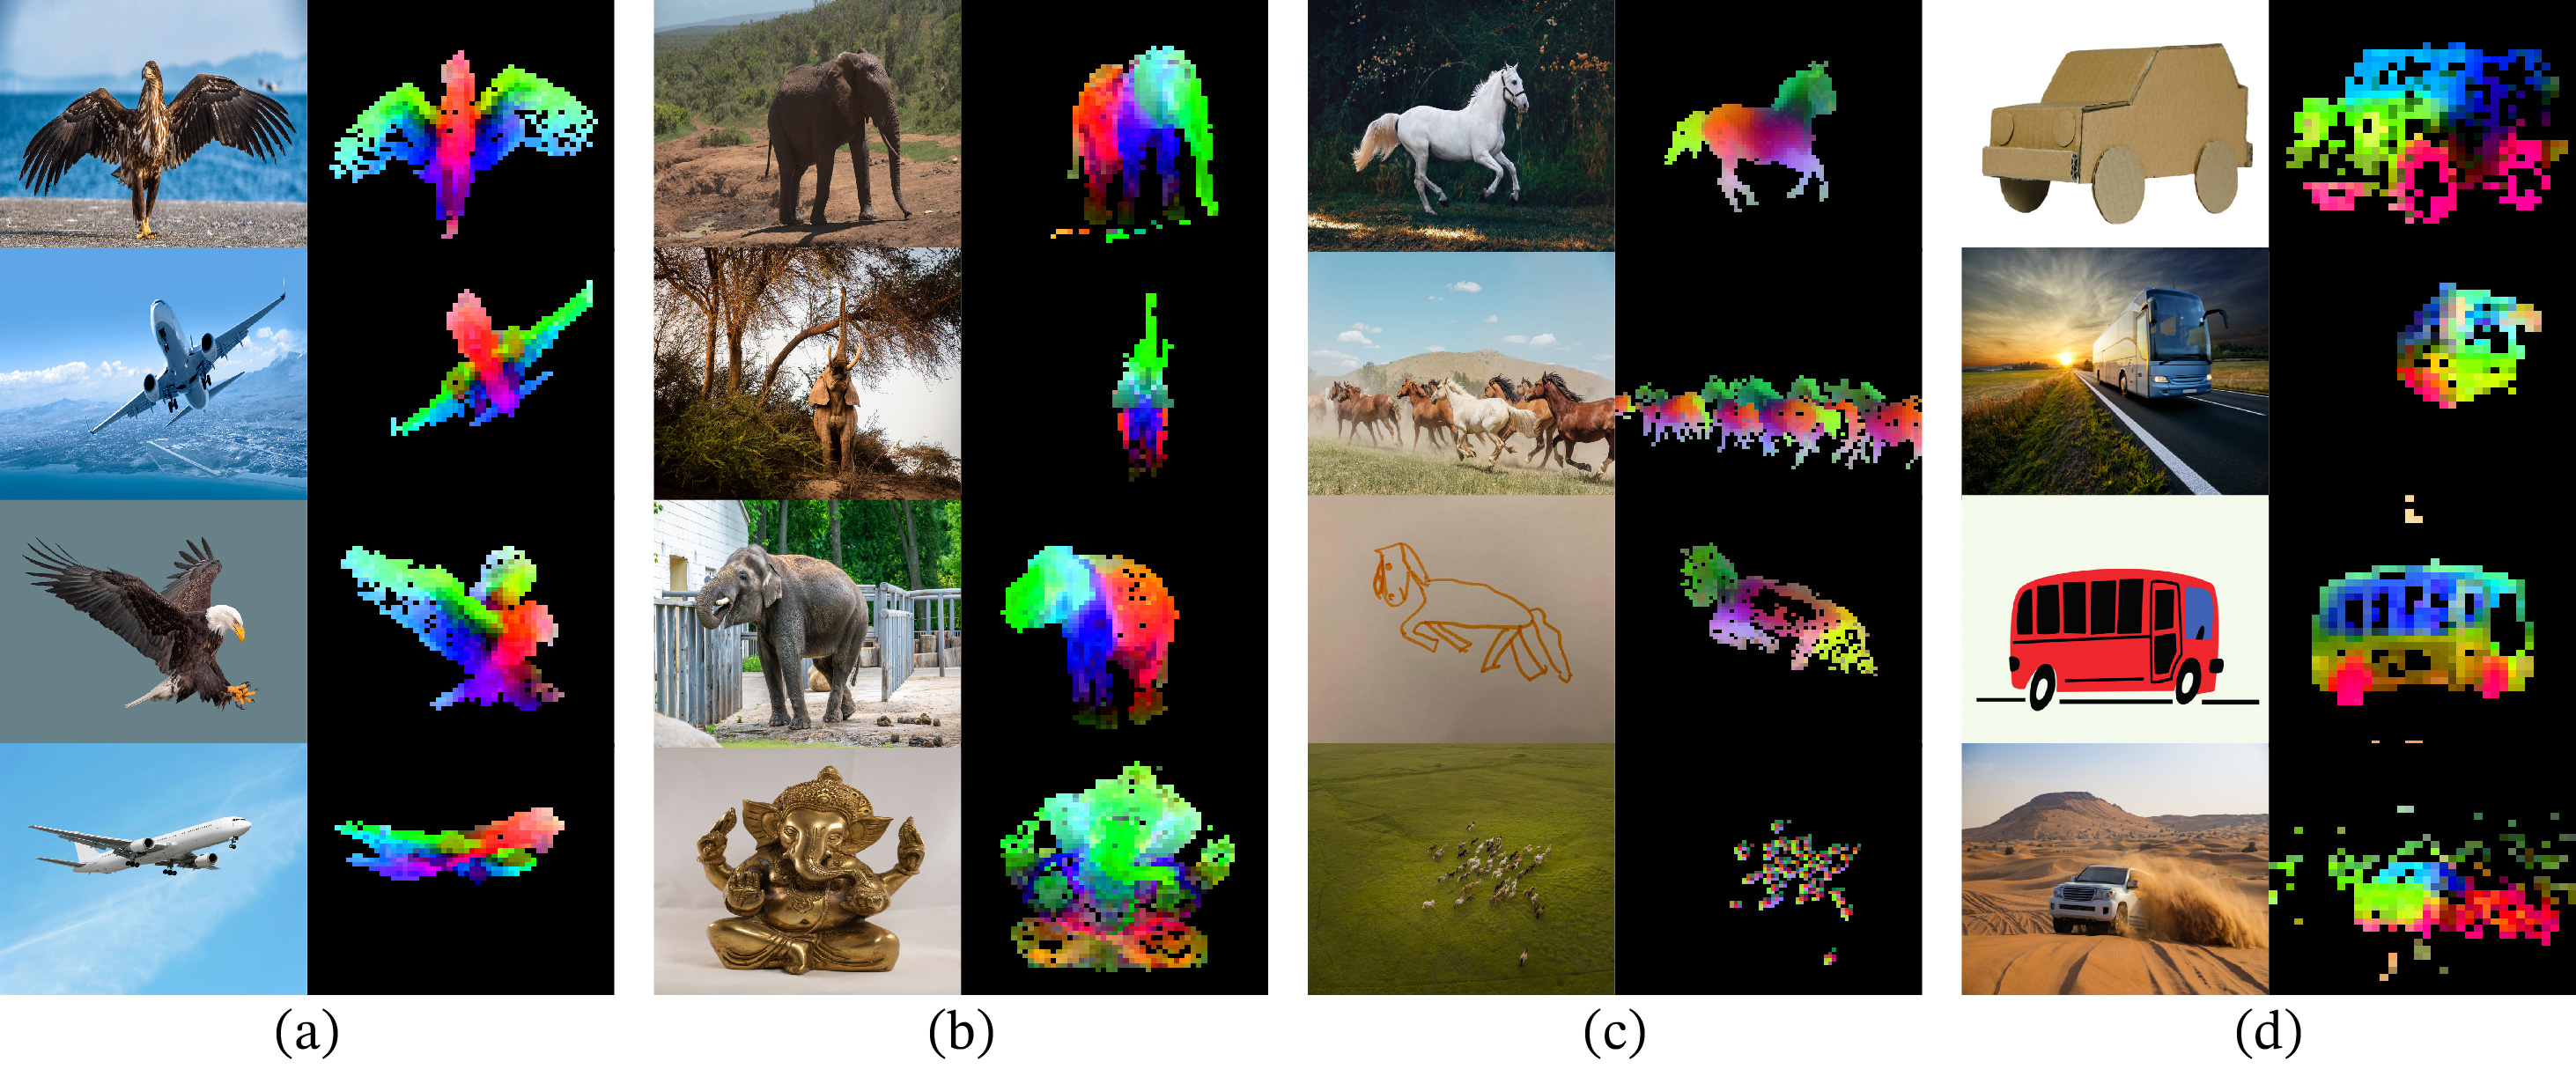
\includegraphics[width=\columnwidth,height=3.0cm,keepaspectratio]{figures/fig1.2.jpg}\\[0.05cm]
            {\tiny \textbf{Hình 1:} PCA visualization của patch features: DINOv2 nhận ra các vùng tương ứng giữa những ảnh liên quan dù thay đổi tư thế, phong cách}
            \vspace{0.15cm}
            \begin{tikzpicture}
                \node[draw=uetblue,fill=uetgold!25,rounded corners,inner sep=7pt,
                      text width=6.2cm,align=center,font=\small] {
                    \textbf{DINOv2 = SSL ở quy mô lớn}\\
                    $\Downarrow$\\
                    \textbf{Visual Foundation Model}\\
                    \footnotesize Không nhãn, không caption --- học thuần từ ảnh
                };
            \end{tikzpicture}
        \end{column}
    \end{columns}
\end{frame}

% ============================================================
% SLIDE 5: TIẾN TRÌNH SSL
% ============================================================
\begin{frame}[t,shrink=15]{Tiến trình phát triển SSL \& Vị trí của DINOv2}
    \vspace{0.1cm}
    \small
    \begin{tabular}{|l|l|p{3.8cm}|p{3.5cm}|}
        \hline
        \rowcolor{uetblue!20}
        \textbf{Giai đoạn} & \textbf{Đại diện} & \textbf{Đặc điểm chính} & \textbf{Hạn chế} \\
        \hline
        Instance discrimination & SimCLR, MoCo & Học tương phản mức ảnh & Chỉ mạnh ở image-level \\
        \hline
        SSL với ViT & DINO & Đặc trưng phân vùng ảnh tự phát & Quy mô dữ liệu hạn chế \\
        \hline
        Masked pretraining & MAE & Che và tái tạo ảnh & Thường cần fine-tune \\
        \hline
        Patch-level SSL & iBOT & DINO + masked image modeling & Khó scale, dữ liệu nhỏ \\
        \hline
        \rowcolor{uetgold!35}
        \textbf{DINOv2} & \textbf{DINOv2} & \textbf{Curated data + SSL recipe + Distillation} & \textbf{Hướng tới frozen features tổng quát} \\
        \hline
    \end{tabular}\\[0.1cm]
    {\tiny \textbf{Bảng 1:} Tiến trình phát triển SSL và vị trí của DINOv2}
    \vspace{0.1cm}
    \begin{columns}[c]
        \begin{column}{0.32\textwidth}
            \begin{exampleblock}{\centering Điểm khác biệt}
                \centering\small
                Giải quyết \textbf{đồng thời}:\\
                chất lượng dữ liệu\\
                + thuật toán SSL\\
                + kỹ thuật scale
            \end{exampleblock}
        \end{column}
        \begin{column}{0.65\textwidth}
            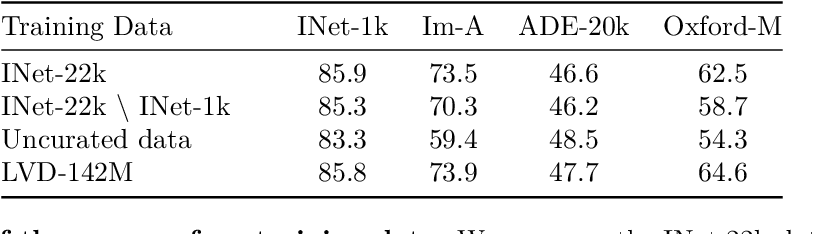
\includegraphics[width=\columnwidth,height=2.0cm,keepaspectratio]{figures/table1.png}
            {\tiny \textbf{Bảng 2:} So sánh nguồn dữ liệu pretraining: LVD-142M cho kết quả vượt trội}
        \end{column}
    \end{columns}
\end{frame}

% ============================================================
\section{Phương pháp DINOv2}
% ============================================================

% ============================================================
% SLIDE 6: TỔNG QUAN PIPELINE
% ============================================================
\begin{frame}[t,shrink=15]{Tổng quan Pipeline DINOv2}
    \begin{center}
    \begin{tikzpicture}[
        box/.style={draw=uetblue,fill=uetblue!12,rounded corners=4pt,
                    minimum width=2.1cm,minimum height=1.4cm,align=center,
                    font=\small,text width=2cm},
        arrow/.style={-{Stealth[length=5pt]},line width=1.5pt,uetblue}
    ]
        \node[box] (d) {\textbf{1. Dữ liệu}\\LVD-142M\\(curated)};
        \node[box,right=0.6cm of d] (a) {\textbf{2. Kiến trúc}\\ViT\\Student--Teacher};
        \node[box,right=0.6cm of a] (o) {\textbf{3. Objective}\\DINO + iBOT\\+ KoLeo};
        \node[box,right=0.6cm of o] (s) {\textbf{4. Scale}\\FlashAttn\\FSDP};
        \node[box,right=0.6cm of s] (di) {\textbf{5. Distill}\\ViT-g/14\\$\to$ S/B/L};
        \draw[arrow] (d) -- (a);
        \draw[arrow] (a) -- (o);
        \draw[arrow] (o) -- (s);
        \draw[arrow] (s) -- (di);
    \end{tikzpicture}
    \end{center}
    \vspace{0.2cm}
    \begin{columns}[t]
        \begin{column}{0.32\textwidth}
            \begin{alertblock}{Ràng buộc quan trọng}
                \begin{itemize}
                    \item \textbf{Không} dùng nhãn lớp
                    \item \textbf{Không} dùng caption văn bản
                    \item Học thuần từ ảnh thô
                \end{itemize}
            \end{alertblock}
        \end{column}
        \begin{column}{0.32\textwidth}
            \begin{block}{Mục tiêu đầu ra}
                \begin{itemize}
                    \item Frozen backbone dùng ngay
                    \item Tốt cả image \& patch level
                    \item Family: ViT-S/B/L/g
                \end{itemize}
            \end{block}
        \end{column}
        \begin{column}{0.32\textwidth}
            \begin{exampleblock}{Đánh giá chính}
                \begin{itemize}
                    \item Linear probe (frozen)
                    \item Nhiều benchmark: classification, segmentation, depth, video
                \end{itemize}
            \end{exampleblock}
        \end{column}
    \end{columns}
\end{frame}

% ============================================================
% SLIDE 7: LVD-142M
% ============================================================
\begin{frame}[t,shrink=25]{Bước 1: Xây dựng dữ liệu LVD-142M}
    \begin{columns}[t]
        \begin{column}{0.54\textwidth}
            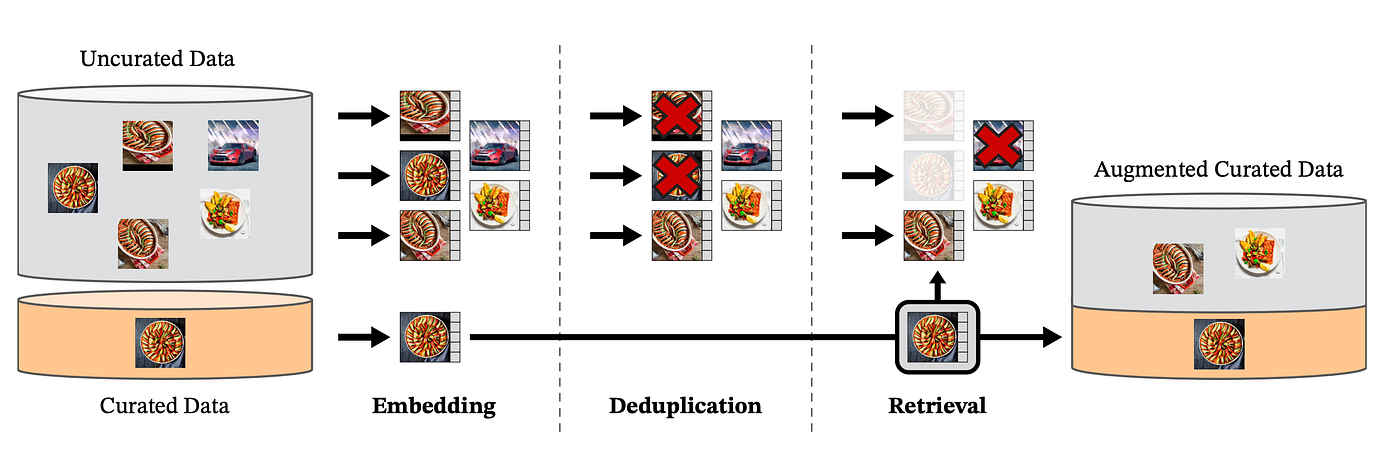
\includegraphics[width=\columnwidth,height=4.2cm,keepaspectratio]{figures/fig1.1.png}
            {\tiny \textbf{Hình 2:} Quy trình xử lý: ảnh thô $\to$ embedding $\to$ dedup $\to$ retrieval $\to$ LVD-142M}
        \end{column}
        \begin{column}{0.43\textwidth}
            \begin{alertblock}{Vấn đề dữ liệu web thô}
                \begin{itemize}
                    \item Nhiễu, trùng lặp nhiều
                    \item Mất cân bằng nội dung
                    \item Không kiểm soát được chất lượng
                \end{itemize}
            \end{alertblock}
            \textbf{Pipeline 3 bước:}
            \begin{enumerate}
                \item \textbf{Embedding}: ViT-H/16 $\to$ vector đặc trưng mỗi ảnh
                \item \textbf{Deduplication}: loại ảnh gần trùng bằng PCA hash + copy detection
                \item \textbf{Retrieval}: tìm $k$-NN gần nhất từ tập curated seed (Faiss + GPU)
            \end{enumerate}
            \vspace{0.2cm}
            \vspace{0.05cm}
            \begin{exampleblock}{Kết quả}
                \alert{142 triệu ảnh} --- đa dạng, cân bằng, ít nhiễu hơn web thô
            \end{exampleblock}
        \end{column}
    \end{columns}
\end{frame}

% ============================================================
% SLIDE 8: KIẾN TRÚC & STUDENT-TEACHER
% ============================================================
\begin{frame}[t,shrink=15]{Bước 2: Kiến trúc ViT \& Cơ chế Student--Teacher}
    \begin{columns}[t]
        \begin{column}{0.48\textwidth}
            \begin{block}{Vision Transformer (ViT)}
                \begin{itemize}
                    \item Ảnh $\to$ \textbf{patch tokens}: biểu diễn từng vùng $14\times14$ px
                    \item \textbf{CLS token}: biểu diễn tổng quát toàn ảnh
                    \item 4 kích thước: ViT-\textbf{S}/\textbf{B}/\textbf{L}/\textbf{g} với patch size 14
                \end{itemize}
            \end{block}
            \vspace{0.2cm}
            \begin{block}{CLS token vs Patch tokens}
                \small
                \begin{tabular}{ll}
                    \textbf{CLS token} & $\to$ classification, retrieval \\
                    \textbf{Patch tokens} & $\to$ segmentation, depth \\
                \end{tabular}\\[0.15cm]
                DINOv2 tối ưu \alert{cả hai loại} trong cùng một backbone
            \end{block}
        \end{column}
        \begin{column}{0.48\textwidth}
            \begin{block}{Cơ chế Student--Teacher}
                \begin{itemize}
                    \item \textbf{Student}: nhận nhiều crops khác nhau $\to$ cập nhật bằng gradient
                    \item \textbf{Teacher}: EMA của student $\to$ tạo target ổn định
                    \[\theta_t \leftarrow m\,\theta_t + (1-m)\,\theta_s\]
                    \item Không có gradient nào chạy qua teacher
                \end{itemize}
            \end{block}
            \vspace{0.2cm}
            \begin{exampleblock}{Trực giác}
                Dù nhìn các crop \textbf{khác nhau} của cùng một ảnh, student phải học biểu diễn \textbf{nhất quán} --- teacher làm ``giám khảo'' ổn định
            \end{exampleblock}
        \end{column}
    \end{columns}
\end{frame}

% ============================================================
% SLIDE 9: OBJECTIVE
% ============================================================
\begin{frame}[t,shrink=15]{Bước 3: Objective Huấn luyện Tự giám sát}
    \begin{columns}[t]
        \begin{column}{0.31\textwidth}
            \begin{block}{DINO Loss\\(Image-level)}
                \small
                \begin{itemize}
                    \item CLS token student\\khớp với teacher
                    \item Cross-entropy\\$p_s$ vs $p_t$
                    \item Sinkhorn-Knopp\\centering
                \end{itemize}
                \vspace{0.1cm}
                \centering$\mathcal{L}_\text{DINO} = -\sum p_t \log p_s$
            \end{block}
        \end{column}
        \begin{column}{0.31\textwidth}
            \begin{block}{iBOT Loss\\(Patch-level)}
                \small
                \begin{itemize}
                    \item Mask ngẫu nhiên\\các patch của student
                    \item Student đoán phân\\phối patch bị che
                    \item Head \textbf{tách biệt}\\với DINO head
                \end{itemize}
                \vspace{0.1cm}
                \centering$\mathcal{L}_\text{iBOT} = -\sum_i p_{ti}\!\log p_{si}$
            \end{block}
        \end{column}
        \begin{column}{0.31\textwidth}
            \begin{block}{KoLeo\\Regularizer}
                \small
                \begin{itemize}
                    \item Trải đều embedding\\trong không gian
                    \item Phạt khi features\\tụ quá gần nhau
                    \item Hữu ích cho\\retrieval tasks
                \end{itemize}
                \vspace{0.1cm}
                \centering$\mathcal{L}_\text{koleo} = -\frac{1}{n}\sum_i \log d_{n,i}$
            \end{block}
        \end{column}
    \end{columns}
    \vspace{0.1cm}
    \begin{columns}[c]
        \begin{column}{0.4\textwidth}
            \begin{tikzpicture}
                \node[draw=uetblue,fill=uetgold!25,rounded corners,inner sep=6pt,
                      text width=5.5cm,align=center] {
                    \small$\mathcal{L} = \mathcal{L}_\text{DINO} + \mathcal{L}_\text{iBOT} + \lambda\,\mathcal{L}_\text{koleo}$\\[2pt]
                    \footnotesize Image-level \textbf{+} patch-level trong cùng backbone
                };
            \end{tikzpicture}
        \end{column}
        \begin{column}{0.56\textwidth}
            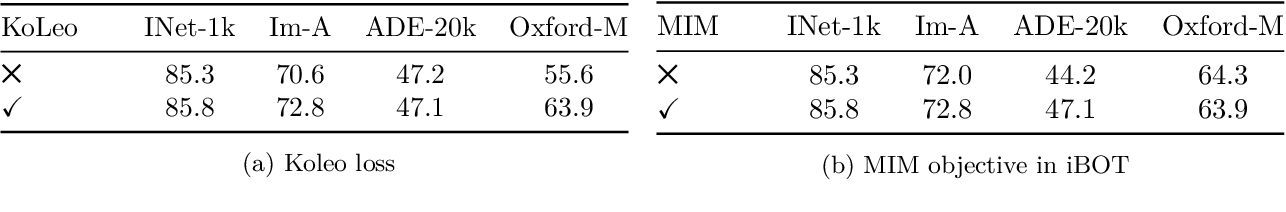
\includegraphics[width=\columnwidth,height=2.0cm,keepaspectratio]{figures/table2.png}
            {\tiny \textbf{Bảng 3:} Ablation: KoLeo cải thiện retrieval; iBOT/MIM giúp dense prediction như segmentation}
        \end{column}
    \end{columns}
\end{frame}

% ============================================================
% SLIDE 10: SCALE & IMPLEMENTATION
% ============================================================
\begin{frame}[t,shrink=15]{Bước 4: Scale \& Kỹ thuật Triển khai}
    \begin{columns}[t]
        \begin{column}{0.52\textwidth}
            \begin{block}{Kỹ thuật tối ưu bộ nhớ \& tốc độ}
                \begin{itemize}
                    \item \textbf{FlashAttention}: attention tiết kiệm bộ nhớ, tăng tốc self-attention trên chuỗi dài
                    \item \textbf{Sequence Packing}: ghép nhiều crop vào một chuỗi dài, block-diagonal attention mask
                    \item \textbf{Efficient Stochastic Depth}: bỏ qua trực tiếp computation của residual bị drop
                    \item \textbf{FSDP}: shard model + optimizer qua nhiều GPU, train được ViT-g $>$1B params
                \end{itemize}
            \end{block}
            \vspace{0.2cm}
            \begin{exampleblock}{Hiệu quả so với iBOT baseline}
                \centering Nhanh \alert{gấp 2×} \quad Tiết kiệm \alert{3× bộ nhớ} GPU
            \end{exampleblock}
        \end{column}
        \begin{column}{0.45\textwidth}
            \begin{block}{High-Resolution Adaptation}
                \begin{itemize}
                    \item Train chủ yếu ở $224\times224$
                    \item Giai đoạn ngắn cuối: \alert{$518\times518$}
                    \item Chi phí thấp, gần đạt chất lượng full high-res
                \end{itemize}
            \end{block}
            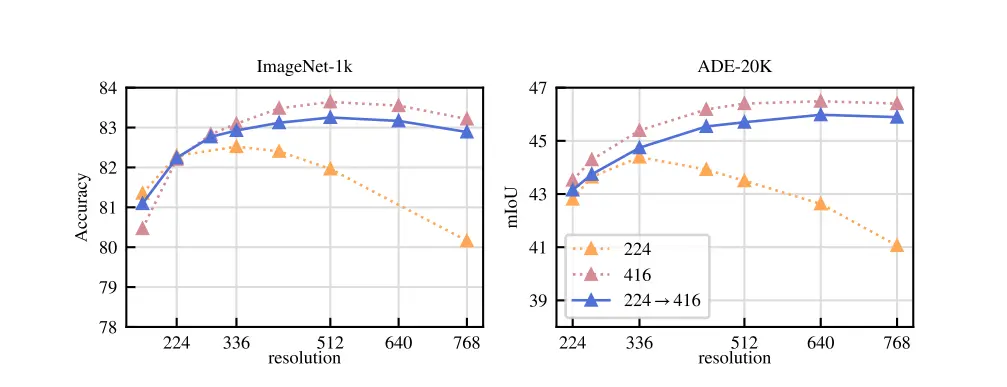
\includegraphics[width=\columnwidth,height=2.8cm,keepaspectratio]{figures/fig1.5.png}
            {\tiny \textbf{Hình 3:} Chuyển sang 518px cuối pretraining: cải thiện cả ImageNet-1k và ADE20K với ít compute hơn}
        \end{column}
    \end{columns}
\end{frame}

% ============================================================
% SLIDE 11: DISTILLATION
% ============================================================
\begin{frame}[t,shrink=15]{Bước 5: Distillation --- Xây dựng Model Family}
    \begin{columns}[t]
        \begin{column}{0.48\textwidth}
            \begin{block}{Tại sao cần Distillation?}
                \begin{itemize}
                    \item Train từng kích thước từ đầu: \alert{rất tốn kém}
                    \item Distillation: model nhỏ \textbf{kế thừa chất lượng} từ ViT-g/14
                    \item ViT-g/14 (teacher cố định) $\to$ student học tái tạo output của teacher
                    \item EMA của student được giữ làm model cuối
                \end{itemize}
            \end{block}
            \vspace{0.2cm}
            \begin{block}{Family model công bố (pretrained)}
                \small
                \begin{tabular}{lcc}
                    \toprule
                    \textbf{Model} & \textbf{Params} & \textbf{Patch} \\
                    \midrule
                    ViT-S/14 & $\sim$21M & 14px \\
                    ViT-B/14 & $\sim$86M & 14px \\
                    ViT-L/14 & $\sim$307M & 14px \\
                    ViT-g/14 & $\sim$1.1B & 14px \\
                    \bottomrule
                \end{tabular}
            \end{block}
        \end{column}
        \begin{column}{0.48\textwidth}
            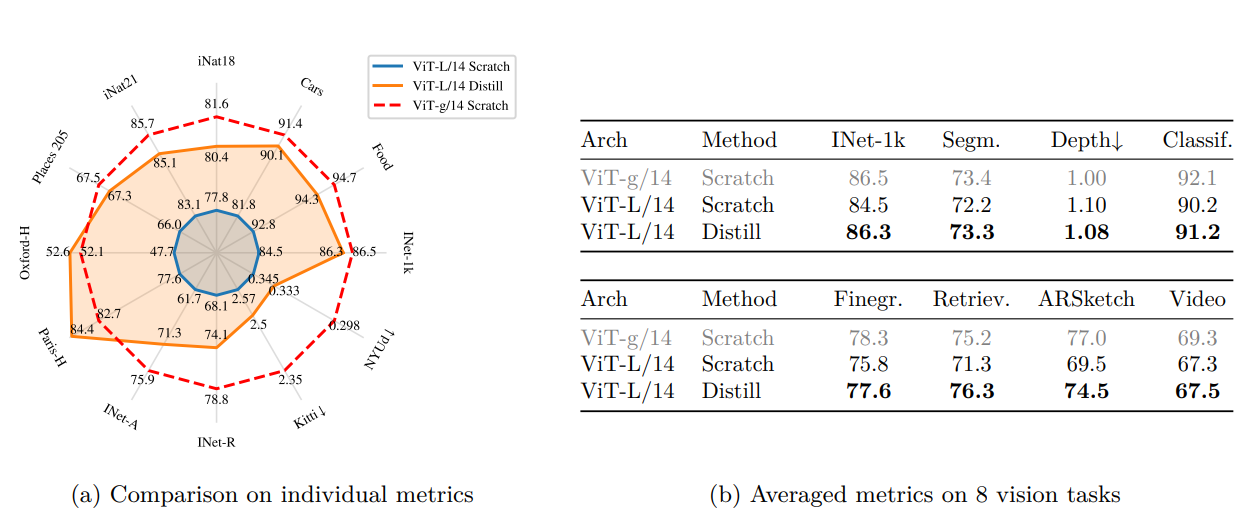
\includegraphics[width=\columnwidth,height=3.8cm,keepaspectratio]{figures/fig1.6.png}
            {\tiny \textbf{Hình 4:} ViT-L/14 distilled từ ViT-g/14 vượt ViT-L/14 train từ scratch trên nhiều benchmark}
            \vspace{0.1cm}
            \begin{exampleblock}{Kết quả nổi bật}
                \small ViT-L/14 \textbf{distilled} luôn vượt ViT-L/14 \textbf{train từ đầu} $\to$ distillation không chỉ tiết kiệm compute mà còn \textbf{cải thiện chất lượng}
            \end{exampleblock}
        \end{column}
    \end{columns}
\end{frame}

% ============================================================
% SLIDE 12: KẾT QUẢ TỪ PAPER
% ============================================================
\begin{frame}[t,shrink=15]{Kết quả từ Paper: DINOv2 so với SOTA}
    \begin{columns}[t]
        \begin{column}{0.52\textwidth}
            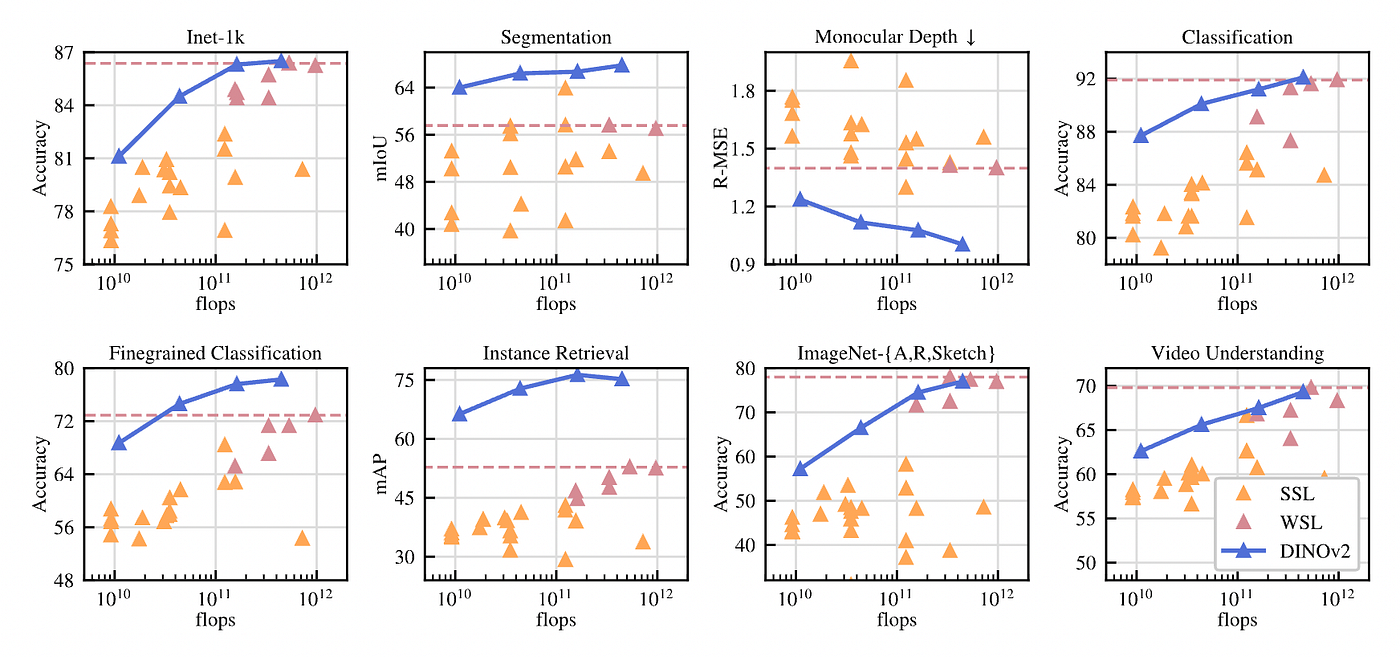
\includegraphics[width=\columnwidth,height=2.6cm,keepaspectratio]{figures/fig1.3.png}
            {\tiny \textbf{Hình 5:} Scaling performance: DINOv2 cải thiện mạnh theo kích thước model, đạt mức cạnh tranh với weakly-supervised}
            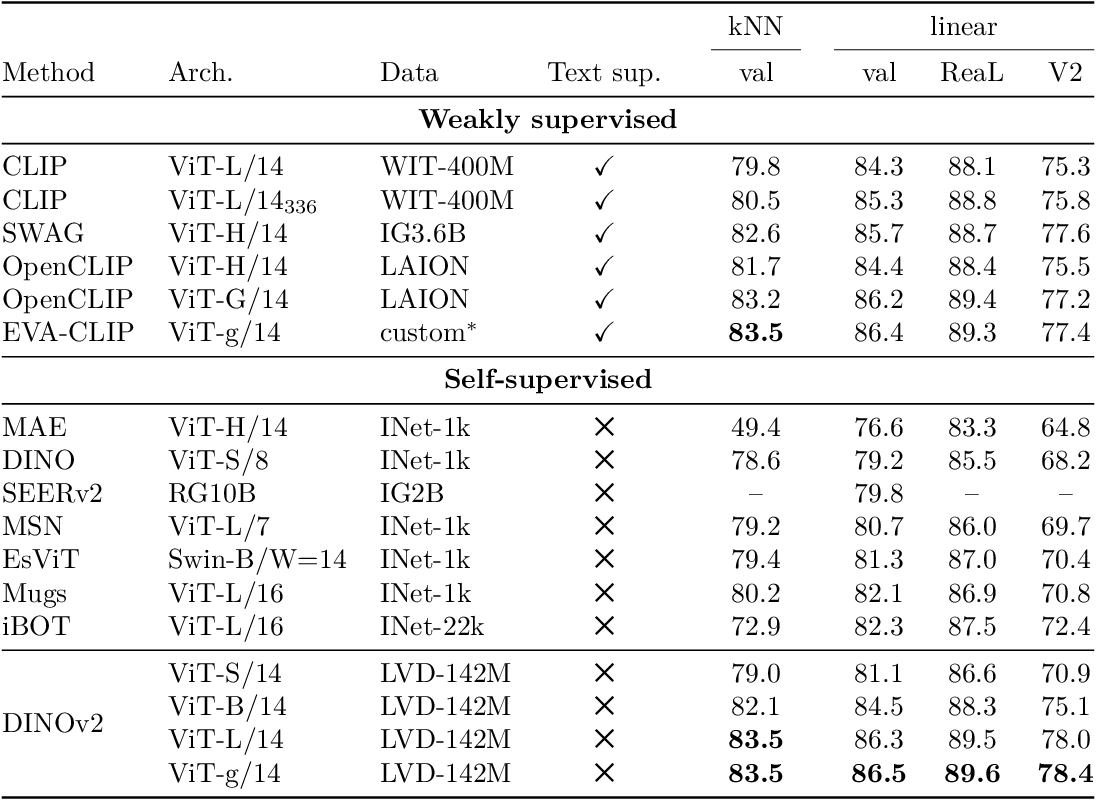
\includegraphics[width=\columnwidth,height=2.0cm,keepaspectratio]{figures/table4.png}
            {\tiny \textbf{Bảng 4:} Linear evaluation ImageNet-1k: DINOv2 ViT-g đạt 86.5\%, ngang OpenCLIP và EVA-CLIP}
        \end{column}
        \begin{column}{0.45\textwidth}
            \begin{block}{Kết quả chính (Frozen backbone)}
                \small
                \begin{tabular}{lc}
                    \toprule
                    \textbf{Benchmark} & \textbf{DINOv2-g} \\
                    \midrule
                    ImageNet-1k (linear) & \alert{86.5\%} \\
                    ImageNet-A & \alert{75.9\%} \\
                    iNaturalist 2021 & \alert{85.7\%} \\
                    Kinetics-400 & \alert{78.4\%} \\
                    \midrule
                    ADE20K (mIoU) & \alert{49.0} \\
                    NYUd depth (RMSE) & \alert{0.344} \\
                    \bottomrule
                \end{tabular}
            \end{block}
            \begin{exampleblock}{Kết luận từ paper}
                \small SSL $\approx$ weakly-supervised nếu:\\
                \textbf{dữ liệu curated tốt} + \textbf{scale đủ lớn}
            \end{exampleblock}
            \begin{alertblock}{Điểm đáng chú ý}
                \small Mạnh cả \textbf{image-level} lẫn \textbf{dense tasks} --- điều mà các SSL trước đó không đạt được đồng thời
            \end{alertblock}
        \end{column}
    \end{columns}
\end{frame}

% ============================================================
\section{Thực nghiệm}
% ============================================================

% ============================================================
% SLIDE 13: TN1 SETUP
% ============================================================
\begin{frame}[t,shrink=15]{Thực nghiệm 1: Phân loại ảnh Y tế}
    \begin{columns}[t]
        \begin{column}{0.48\textwidth}
            \begin{block}{Bộ dữ liệu: SkinCancerMNIST (HAM10000)}
                \begin{itemize}
                    \item \textbf{10,015 ảnh} nội soi da liễu
                    \item \textbf{7 lớp bệnh lý}: MEL, NV, BCC,\\AKIEC, BKL, DF, VASC
                    \item Thách thức: \alert{mất cân bằng nghiêm trọng}\\
                          NV $>$67\% \ \ DF/VASC $<$2\%
                    \item Domain hoàn toàn mới với cả hai model
                \end{itemize}
            \end{block}
            \vspace{0.2cm}
            \begin{block}{Siêu tham số}
                \small
                \begin{tabular}{ll}
                    Batch size: & 32 \\
                    Max epochs: & 20 + Early Stopping (patience=5) \\
                    Optimizer: & Adam, LR $= 10^{-3}$ \\
                    Loss: & CrossEntropy \\
                \end{tabular}
            \end{block}
        \end{column}
        \begin{column}{0.48\textwidth}
            \begin{exampleblock}{Phương pháp: Linear Probing}
                \begin{itemize}
                    \item \textbf{Đóng băng hoàn toàn} backbone
                    \item Chỉ train \textbf{1 Linear Head} phía trên
                    \item $\Rightarrow$ Đo trực tiếp \textbf{chất lượng features}
                \end{itemize}
            \end{exampleblock}
            \vspace{0.15cm}
            \textbf{Cấu hình so sánh:}
            \vspace{0.05cm}
            \small
            \begin{tabular}{|l|p{3.8cm}|}
                \hline
                \rowcolor{uetblue!15}
                \textbf{Model} & \textbf{Pretrain} \\
                \hline
                ViT-B/16 & Supervised trên ImageNet-1k (có nhãn) \\
                \hline
                \rowcolor{uetgold!20}
                \textbf{DINOv2-ViT-B/14} & Self-supervised trên LVD-142M (\textbf{không nhãn}) \\
                \hline
            \end{tabular}
        \end{column}
    \end{columns}
\end{frame}

% ============================================================
% SLIDE 14: TN1 RESULTS
% ============================================================
\begin{frame}[t,shrink=20]{TN1: Kết quả Phân loại ảnh}
    \begin{columns}[t]
        \begin{column}{0.48\textwidth}
            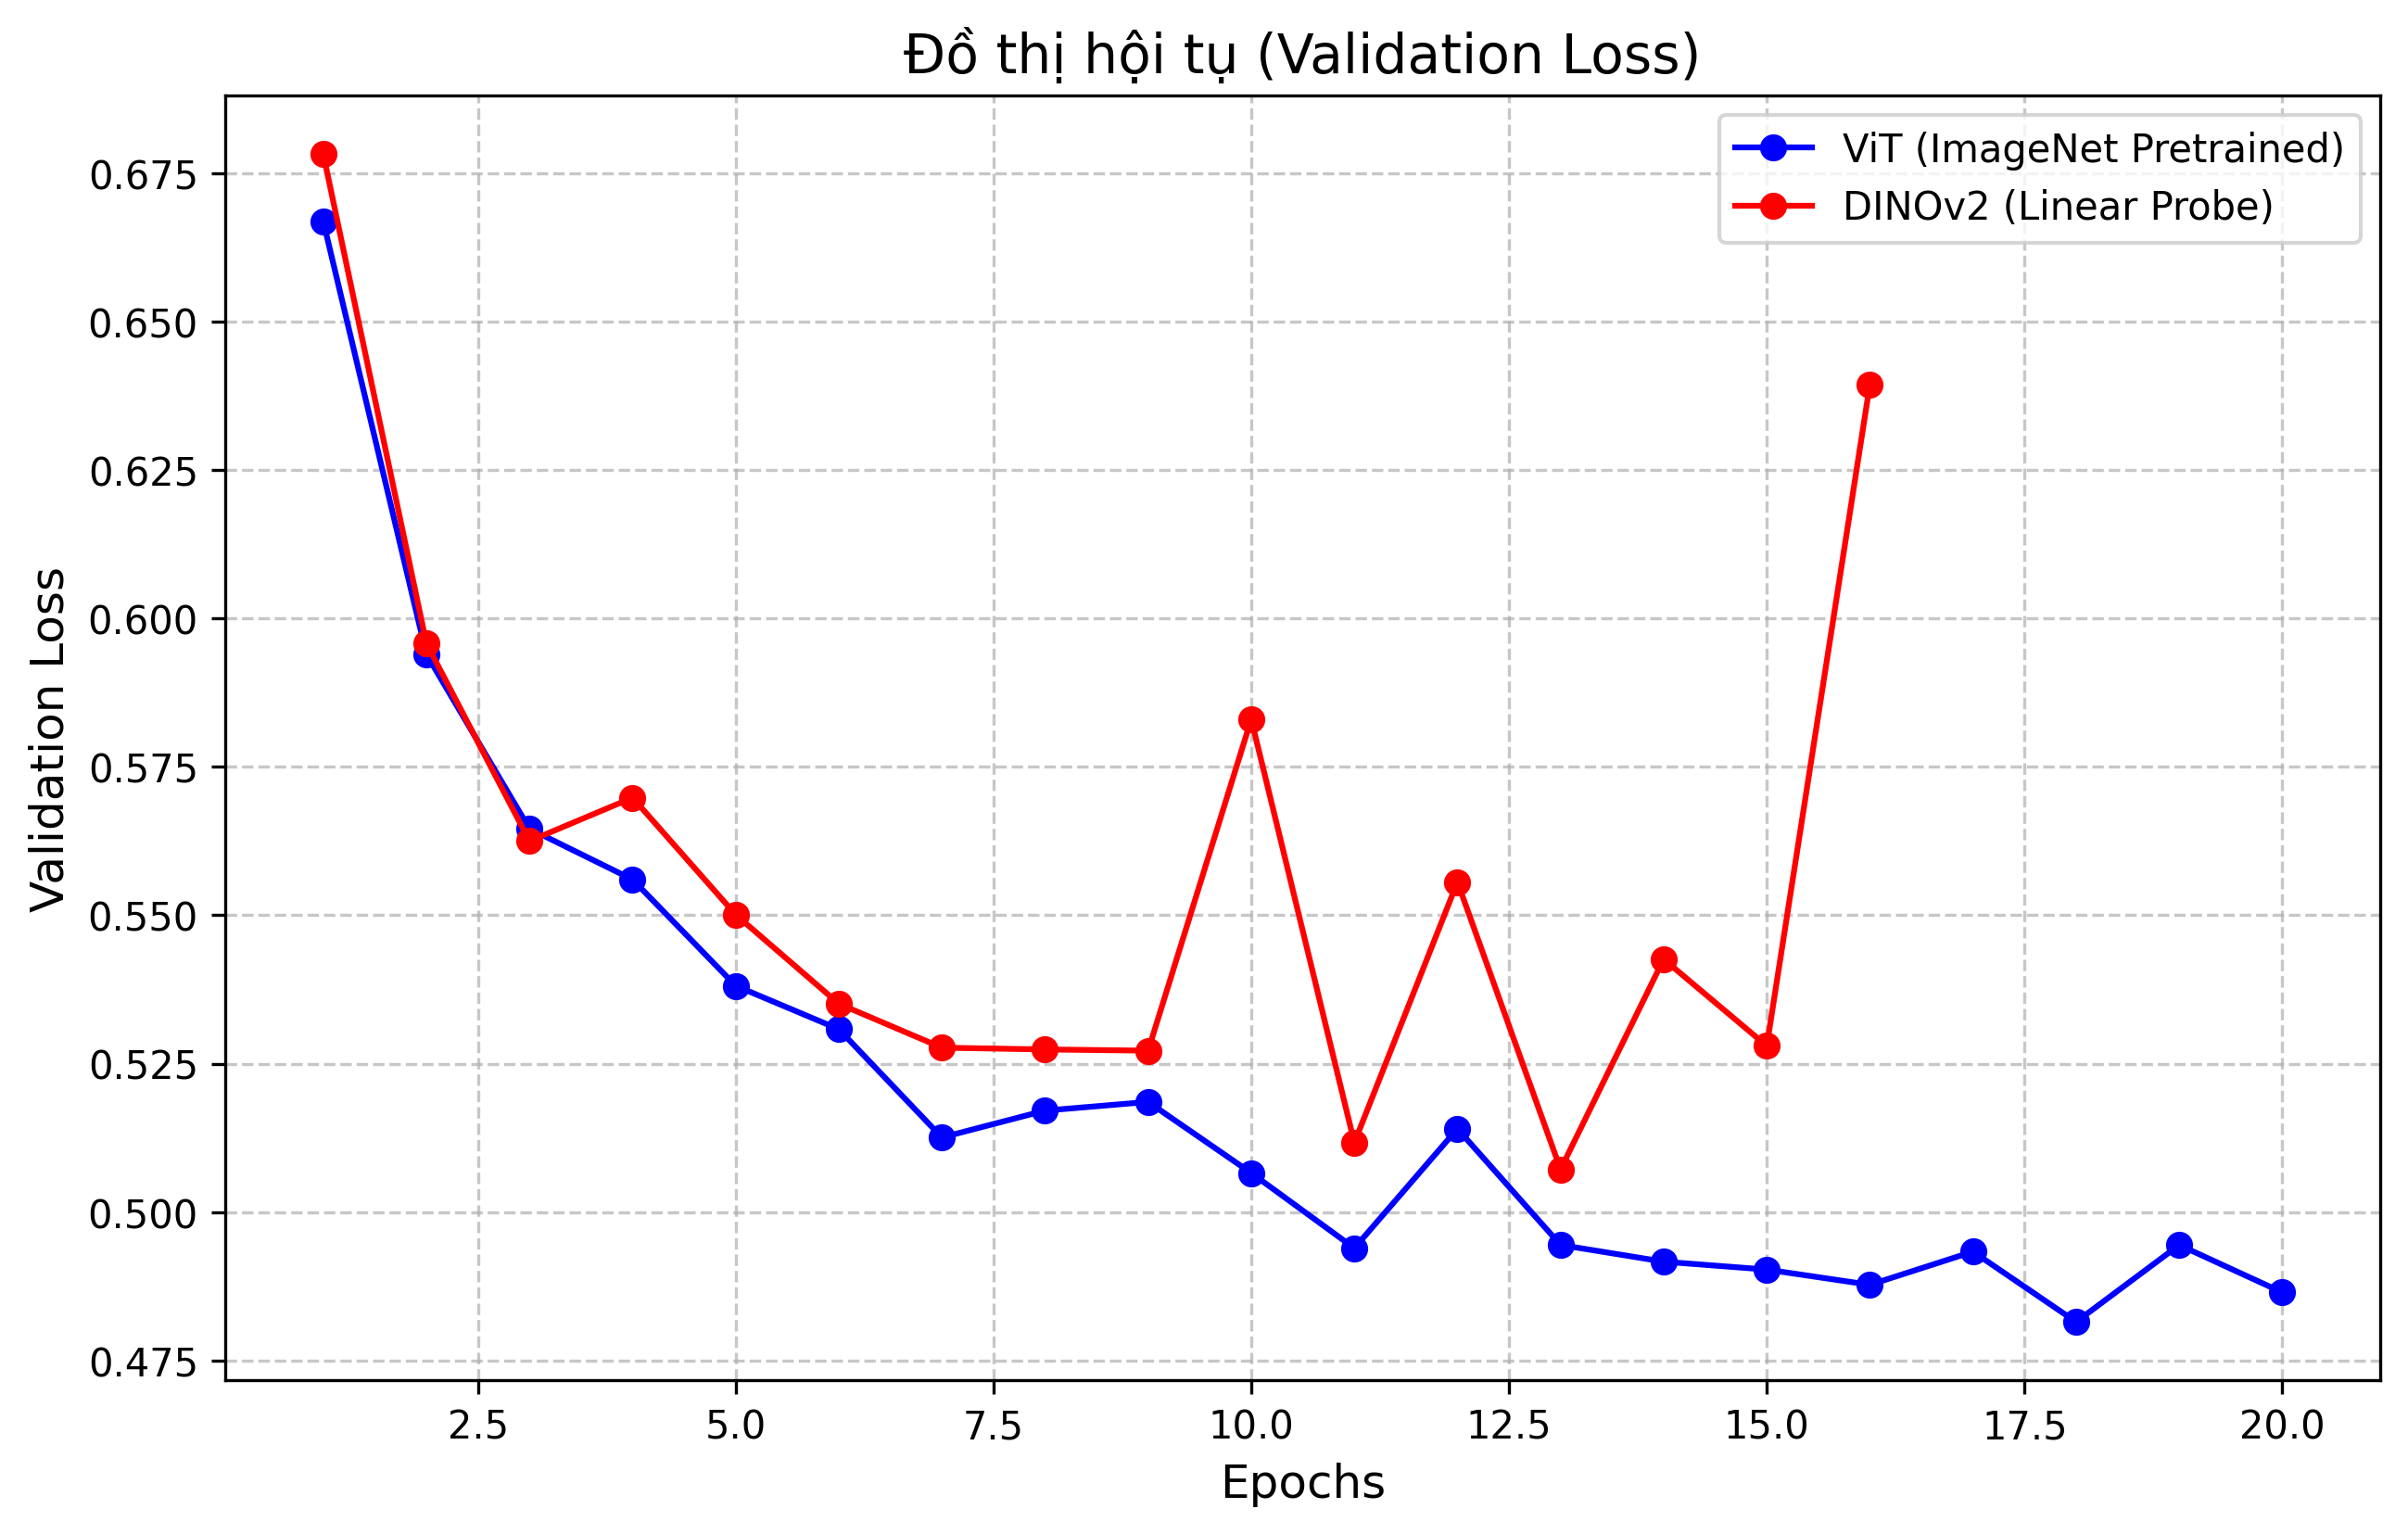
\includegraphics[width=\columnwidth,height=2.5cm,keepaspectratio]{figures/convergence.png}\\
            {\tiny \textbf{Hình 6:} Tốc độ hội tụ (Validation Loss): DINOv2 (đỏ) ổn định và nhanh hơn từ đầu}\\[0.2cm]
            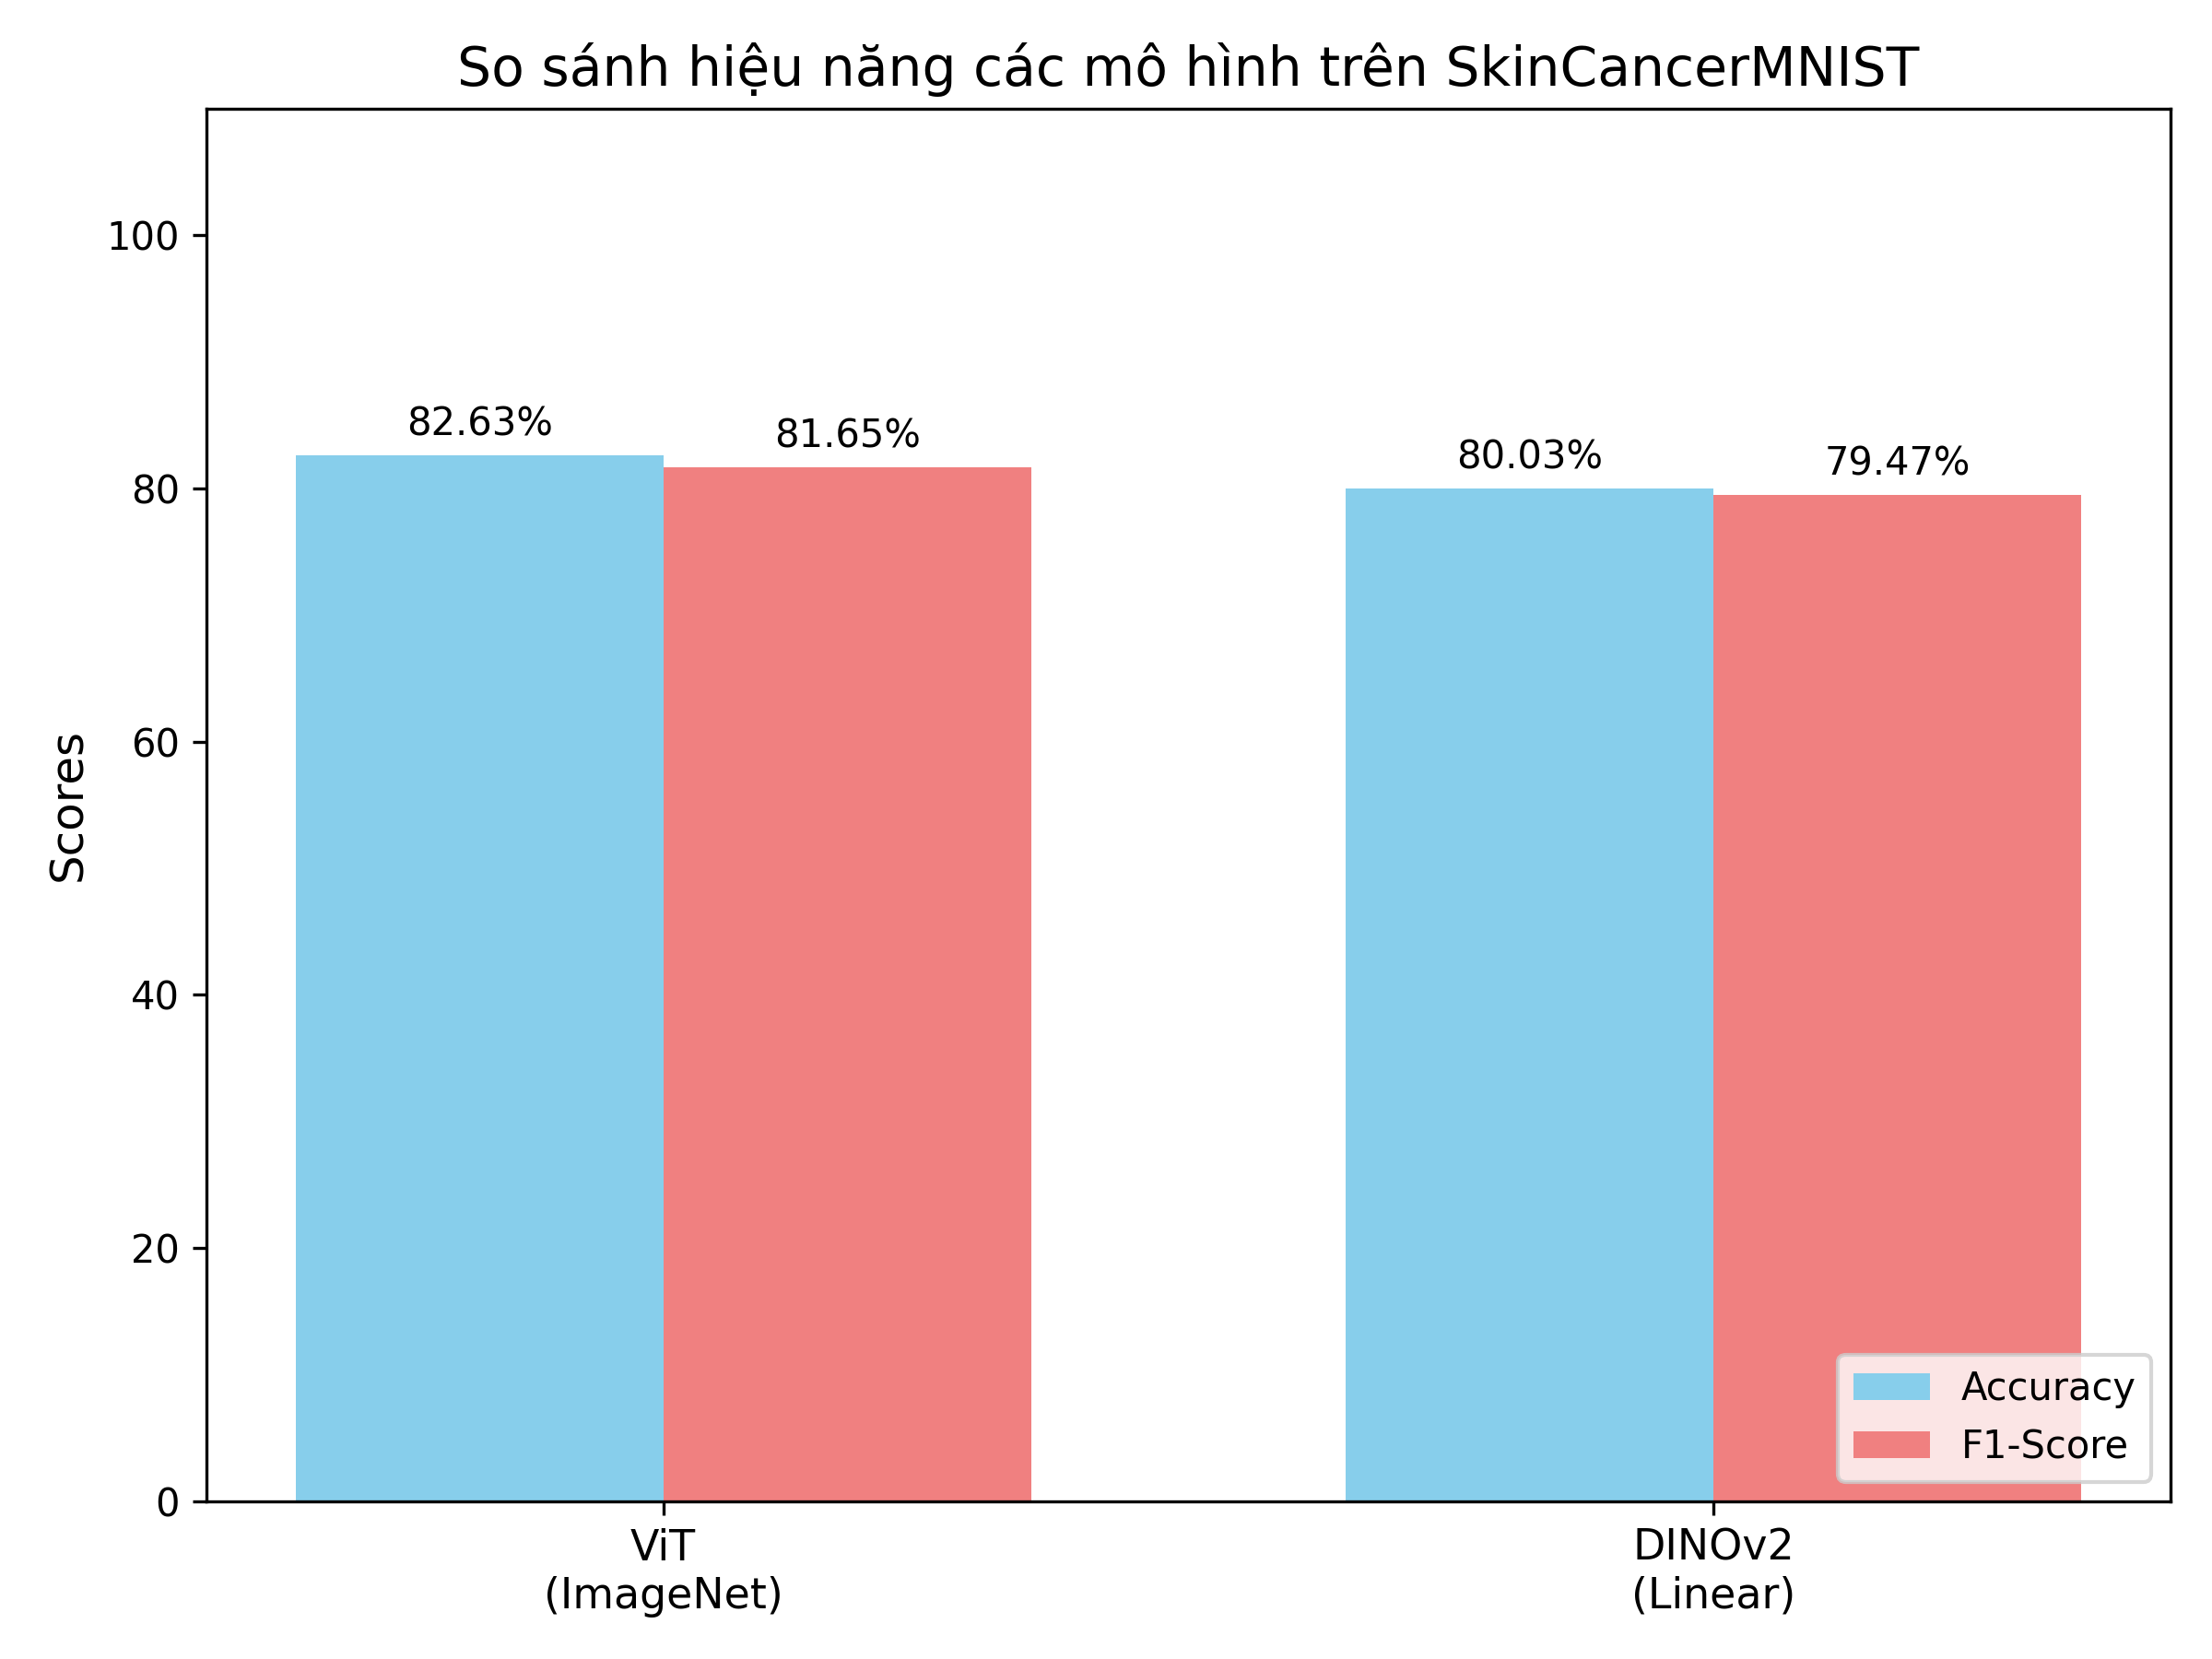
\includegraphics[width=\columnwidth,height=2.4cm,keepaspectratio]{figures/performance_bar.png}\\
            {\tiny \textbf{Hình 7:} So sánh Accuracy và F1-Score trên tập Test}
        \end{column}
        \begin{column}{0.48\textwidth}
            \begin{block}{Kết quả trên tập Test}
                \small
                \begin{tabular}{lcc}
                    \toprule
                    \textbf{Model} & \textbf{Accuracy} & \textbf{F1-Score} \\
                    \midrule
                    ViT-B/16 (supervised) & 82.63\% & 81.65\% \\
                    \rowcolor{uetgold!25}
                    \textbf{DINOv2} (SSL) & \textbf{80.03\%} & \textbf{79.47\%} \\
                    \bottomrule
                \end{tabular}
            \end{block}
            \begin{exampleblock}{Nhận xét quan trọng}
                \small
                \begin{itemize}
                    \item Chênh lệch chỉ \alert{$\approx 2.6\%$} mặc dù DINOv2 \textbf{chưa từng thấy nhãn nào} khi pretrain
                    \item DINOv2 hội tụ nhanh hơn và ổn định hơn trên domain mới (ảnh y tế)
                    \item ViT-B/16 bị \textit{domain-shift}: shape bias học từ ImageNet không khớp hoàn toàn với ảnh nội soi
                \end{itemize}
            \end{exampleblock}
            \begin{alertblock}{Hạn chế chung}
                \small Cả hai nhầm lẫn DF/VASC vào NV do mất cân bằng dữ liệu
            \end{alertblock}
        \end{column}
    \end{columns}
\end{frame}

% ============================================================
% SLIDE 15: TN1 CONFUSION MATRIX
% ============================================================
\begin{frame}[t,shrink=15]{TN1: Phân tích Ma trận Nhầm lẫn}
    \begin{columns}[c]
        \begin{column}{0.47\textwidth}
            \centering
            {\small\textbf{DINOv2 (Self-Supervised)}}\\[0.1cm]
            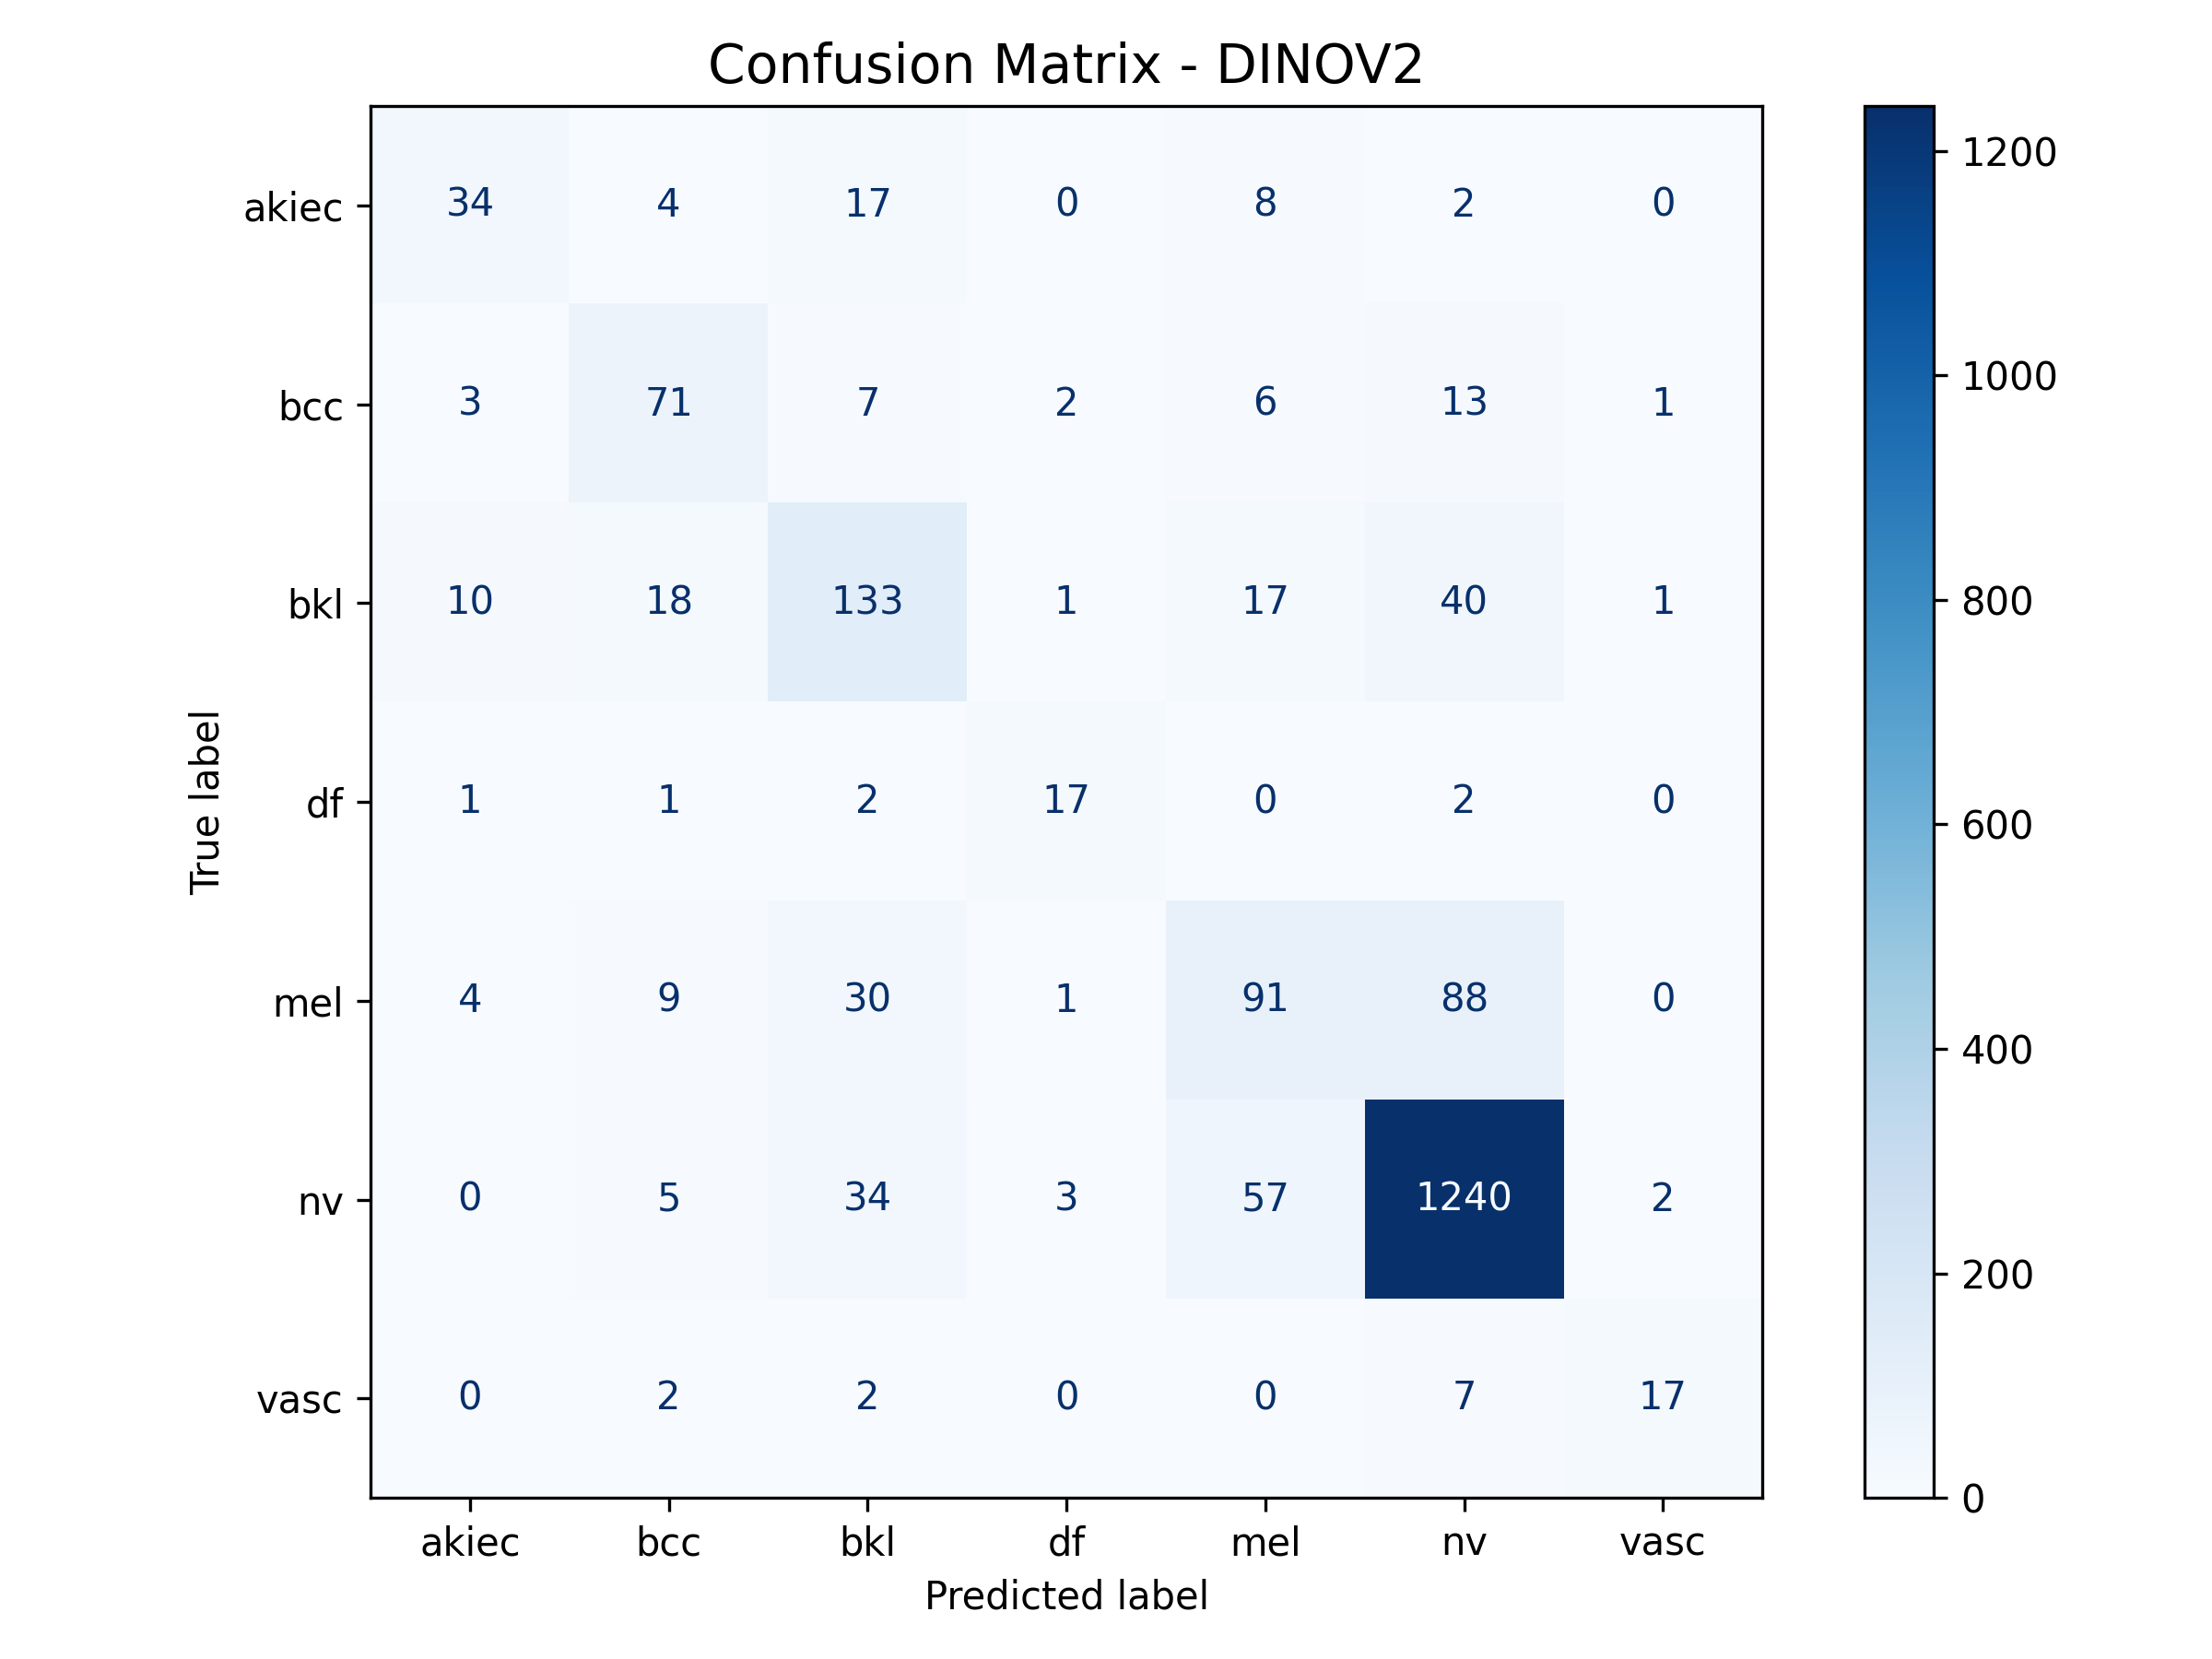
\includegraphics[width=\columnwidth,height=4.0cm,keepaspectratio]{figures/confusion_matrix_dinov2.png}\\[0.05cm]
            {\tiny \textbf{Hình 8:} Ma trận nhầm lẫn của DINOv2 (Self-Supervised)}
        \end{column}
        \begin{column}{0.47\textwidth}
            \centering
            {\small\textbf{ViT-B/16 (ImageNet Supervised)}}\\[0.1cm]
            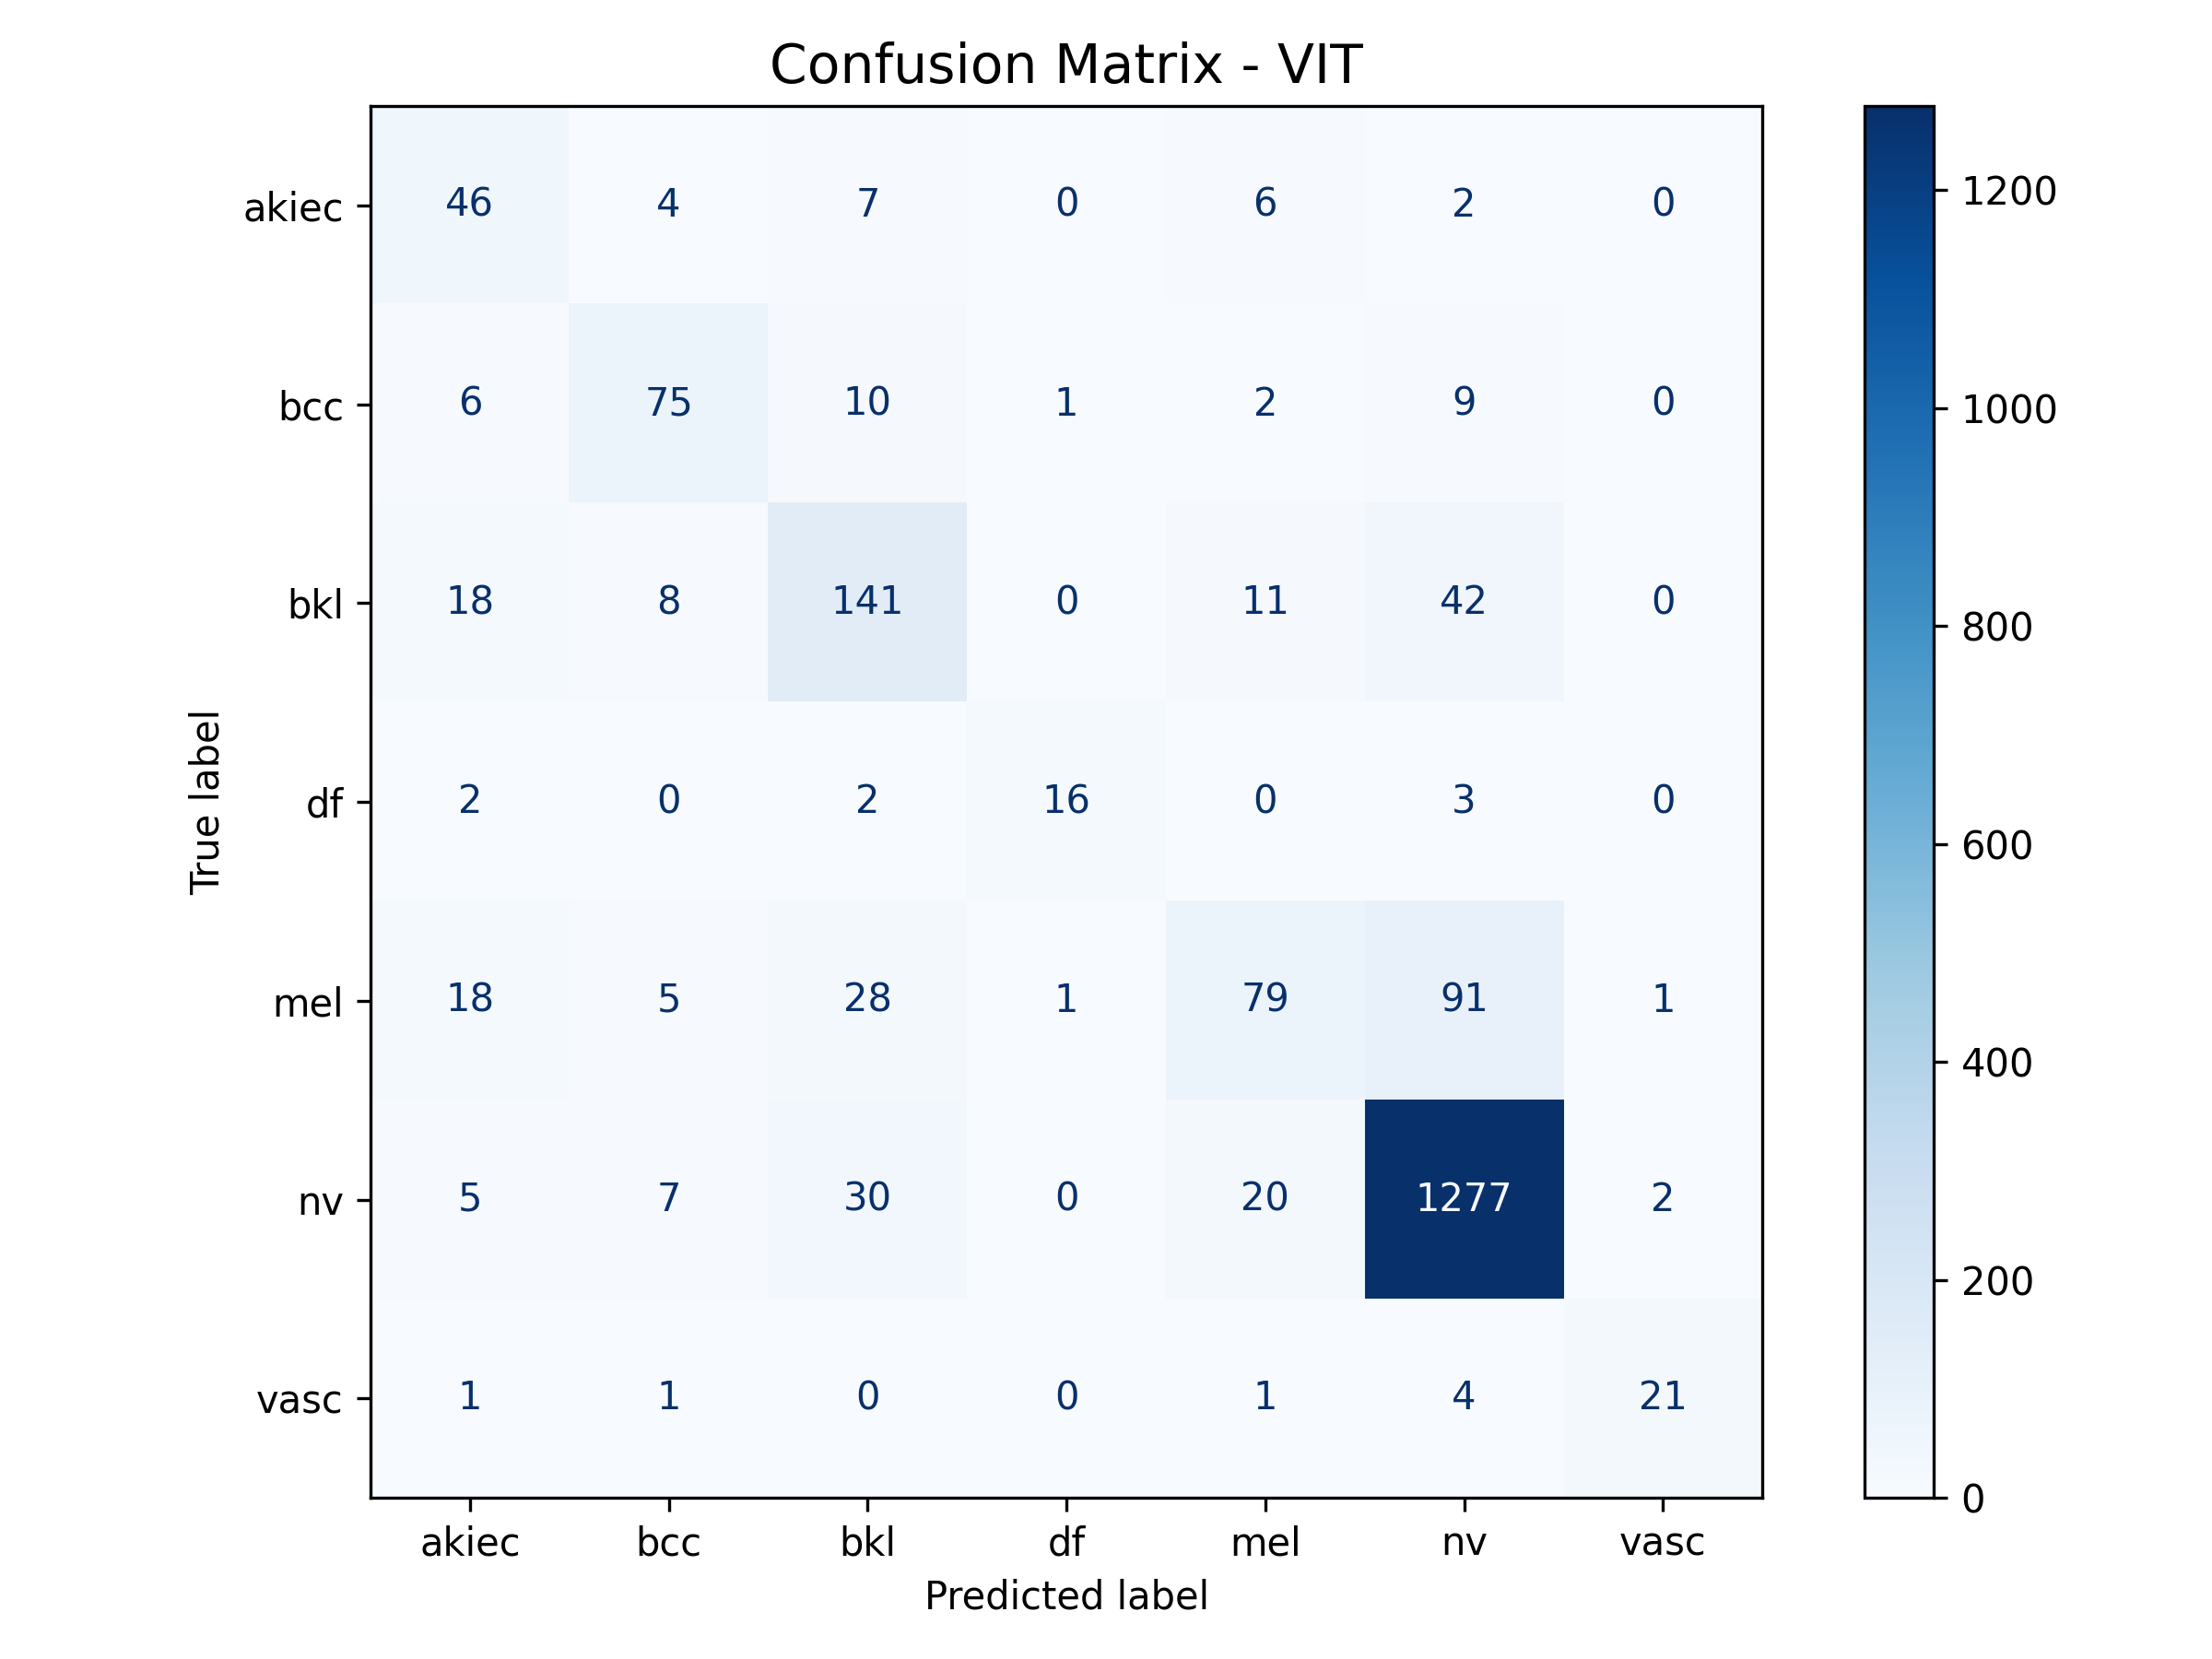
\includegraphics[width=\columnwidth,height=4.0cm,keepaspectratio]{figures/confusion_matrix_vit.png}\\[0.05cm]
            {\tiny \textbf{Hình 9:} Ma trận nhầm lẫn của ViT-B/16 (ImageNet Supervised)}
        \end{column}
    \end{columns}
    \vspace{0.2cm}
    \begin{center}
        \small
        \begin{tabular}{lll}
            \textbf{Điểm chung:} & Nhận diện tốt \textbf{NV} (majority), & yếu với \textbf{DF, VASC} (minority) \\
            \textbf{DINOv2:} & Patch features tốt cho texture cục bộ, & bị nhiễu bởi bóng sáng / lông \\
            \textbf{ViT-B/16:} & Decision boundary cứng từ ImageNet & $\to$ conservative hơn \\
        \end{tabular}
    \end{center}
\end{frame}

% ============================================================
% SLIDE 16: TN2 SETUP
% ============================================================
\begin{frame}[t,shrink=15]{Thực nghiệm 2: Phân đoạn Zero-Shot}
    \begin{columns}[t]
        \begin{column}{0.48\textwidth}
            \begin{block}{Bộ dữ liệu: Oxford-IIIT Pet}
                \begin{itemize}
                    \item 7,349 ảnh chó/mèo, 37 giống
                    \item Annotation \textbf{trimap} 3 lớp:\\
                          \textcolor{red}{\rule{8pt}{8pt}} \textbf{pet} \ / \ \textcolor{blue}{\rule{8pt}{8pt}} \textbf{background} \ / \ \textcolor{successgreen}{\rule{8pt}{8pt}} \textbf{border}
                    \item Split: \textbf{10} ảnh reference, \textbf{150} ảnh eval
                \end{itemize}
            \end{block}
            \vspace{0.15cm}
            \begin{block}{Phương pháp 1: Prototype-based}
                \small 10 ảnh reference $\to$ prototype vector mỗi class $\to$ cosine similarity $\to$ argmax\\
                Chỉ cần \textbf{10 ảnh có nhãn}
            \end{block}
            \vspace{0.1cm}
            \begin{block}{Phương pháp 2: Spherical KMeans}
                \small Clustering patch features ($k$=3) $\to$ greedy IoU matching\\
                \textbf{Không cần nhãn pixel-level nào}
            \end{block}
        \end{column}
        \begin{column}{0.48\textwidth}
            \begin{exampleblock}{Thiết lập: Hoàn toàn Training-free}
                \begin{itemize}
                    \item \alert{Không tính một gradient nào}
                    \item Chỉ dùng \textbf{patch tokens} (frozen)
                    \item Kiểm tra tuyên bố cốt lõi của paper:\\patch features đủ mạnh cho dense task
                \end{itemize}
            \end{exampleblock}
            \vspace{0.2cm}
            \textbf{3 Backbone so sánh (cùng pipeline):}
            \vspace{0.1cm}
            \small
            \begin{tabular}{|l|c|l|}
                \hline
                \rowcolor{uetblue!15}
                \textbf{Backbone} & \textbf{Params} & \textbf{Pretrain} \\
                \hline
                DINOv2-S & $\sim$21M & SSL \\
                \hline
                DINOv2-B & $\sim$86M & SSL \\
                \hline
                ViT-B/16 IN-1K & $\sim$86M & Supervised \\
                \hline
            \end{tabular}
        \end{column}
    \end{columns}
\end{frame}

% ============================================================
% SLIDE 17: TN2 RESULTS
% ============================================================
\begin{frame}[t,shrink=15]{TN2: Kết quả Zero-Shot Segmentation}
    \begin{columns}[t]
        \begin{column}{0.5\textwidth}
            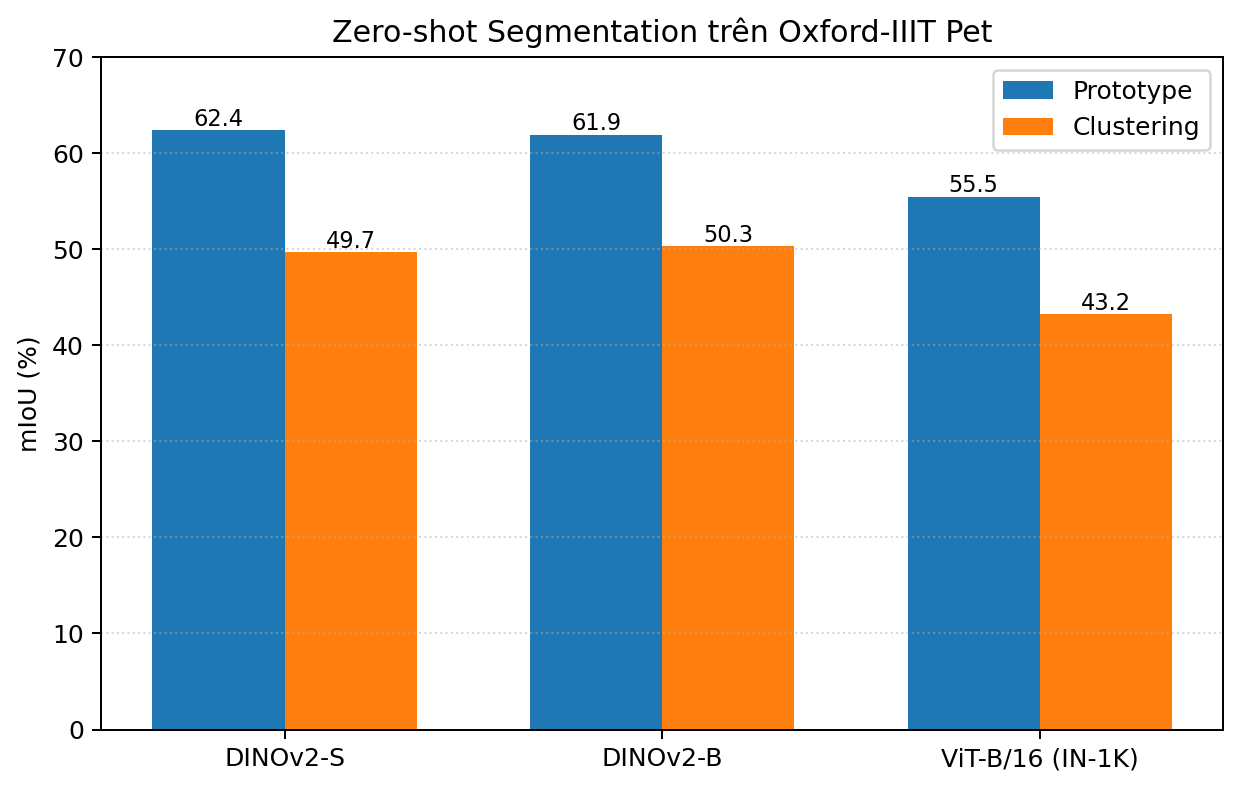
\includegraphics[width=\columnwidth,height=2.4cm,keepaspectratio]{figures/seg_miou_compare.png}
            {\tiny \textbf{Hình 10:} So sánh mIoU: DINOv2 luôn vượt ViT-B/16 ở cả hai phương pháp}
            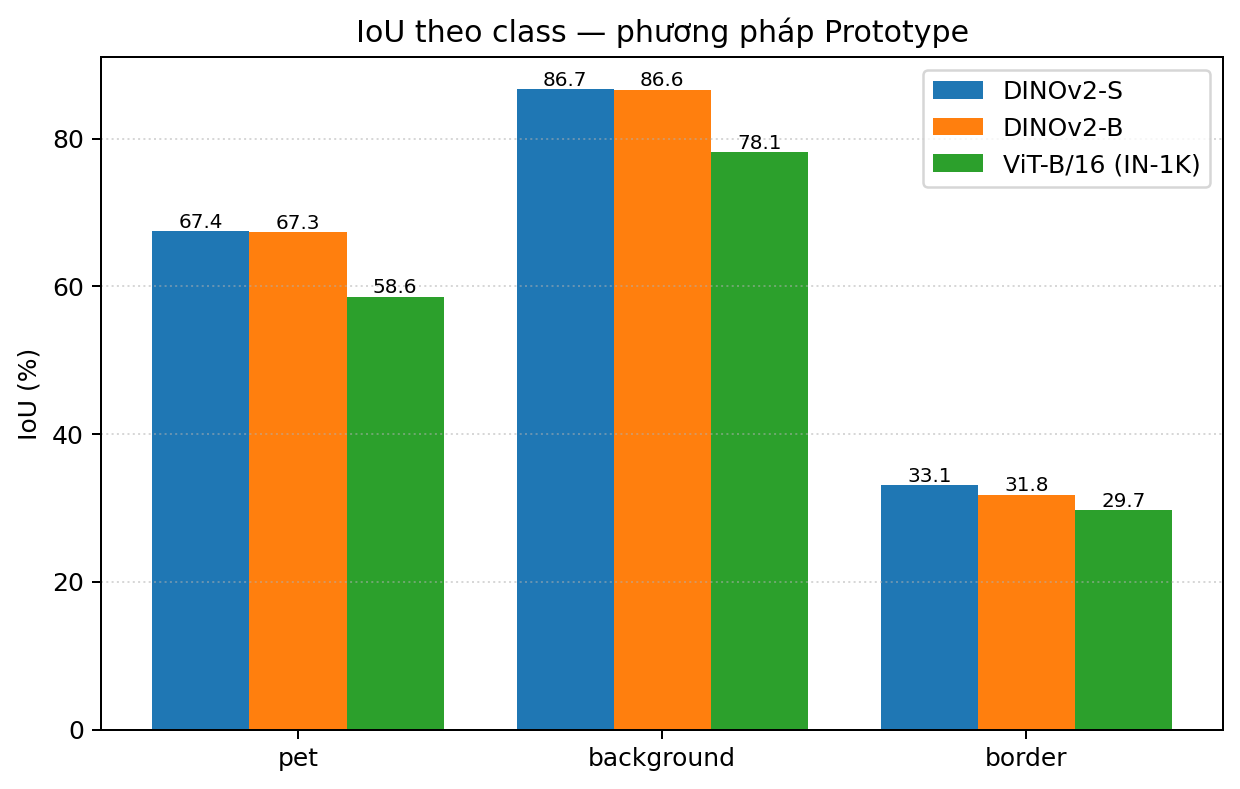
\includegraphics[width=\columnwidth,height=2.3cm,keepaspectratio]{figures/seg_per_class_iou.png}
            {\tiny \textbf{Hình 11:} IoU theo từng class (Prototype): border là điểm yếu chung}
        \end{column}
        \begin{column}{0.47\textwidth}
            \small
            \begin{tabular}{llcc}
                \toprule
                \textbf{Backbone} & \textbf{Method} & \textbf{mIoU} & \textbf{Pix.Acc} \\
                \midrule
                \rowcolor{uetgold!25}
                \textbf{DINOv2-S} & Proto & \textbf{62.39} & \textbf{81.78} \\
                DINOv2-B & Proto & 61.90 & 81.70 \\
                ViT-B/16 & Proto & 55.47 & 75.46 \\
                \midrule
                DINOv2-S & KMeans & 49.69 & 80.19 \\
                \rowcolor{uetgold!25}
                \textbf{DINOv2-B} & \textbf{KMeans} & \textbf{50.31} & \textbf{80.84} \\
                ViT-B/16 & KMeans & 43.24 & 74.92 \\
                \bottomrule
            \end{tabular}
            {\tiny \textbf{Bảng 5:} Kết quả Zero-Shot Segmentation trên Oxford-IIIT Pet}
            \vspace{0.1cm}
            \begin{exampleblock}{3 quan sát quan trọng}
                \small
                \begin{itemize}
                    \item DINOv2 \alert{+7 điểm mIoU} so với ViT cùng kích thước --- khoảng cách lớn hơn nhiều so với TN1
                    \item DINOv2-S (21M) $\approx$ DINOv2-B (86M): nhỏ đủ tốt cho dense task nhẹ
                    \item Class \textit{border} yếu ($\sim$30\%): giới hạn của patch resolution $14\times14$
                \end{itemize}
            \end{exampleblock}
        \end{column}
    \end{columns}
\end{frame}

% ============================================================
% SLIDE 18: TN2 QUALITATIVE
% ============================================================
\begin{frame}[t,shrink=15]{TN2: Phân tích Định tính \& Tính chất Emergence}
    \begin{columns}[t]
        \begin{column}{0.54\textwidth}
            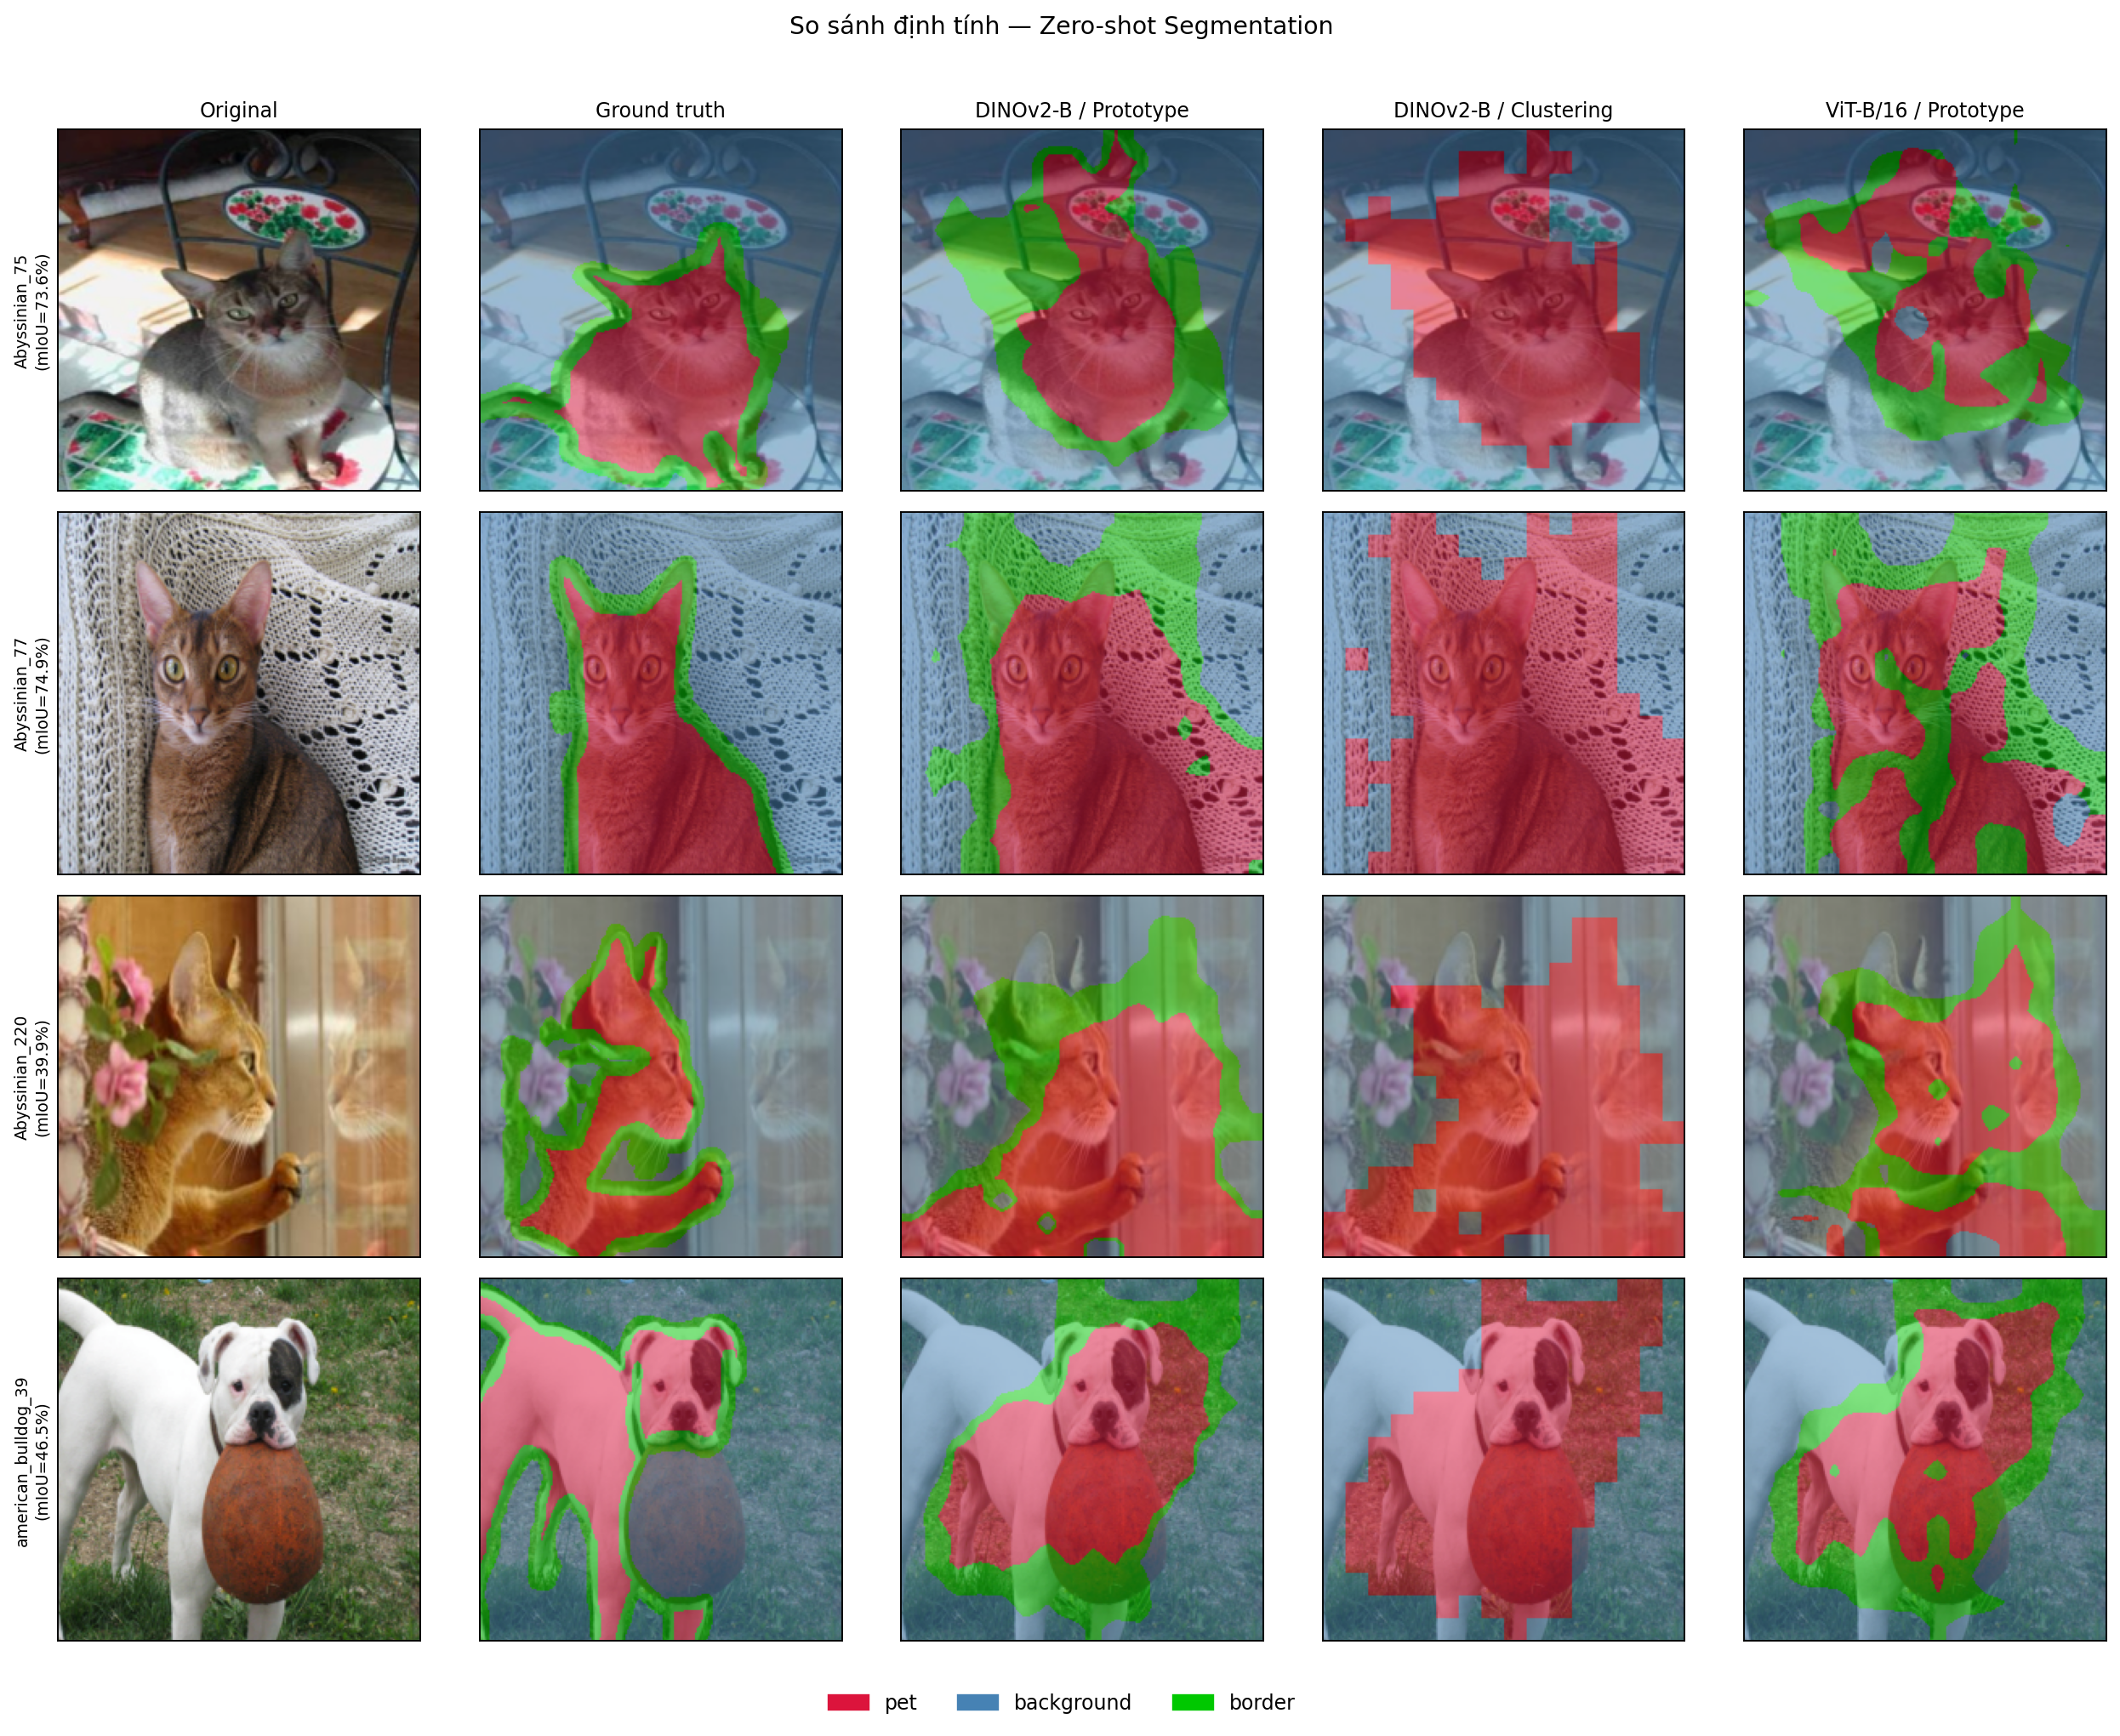
\includegraphics[width=\columnwidth,height=3.8cm,keepaspectratio]{figures/seg_qualitative.png}
            {\tiny \textbf{Hình 12:} Từ trái: Original $|$ Ground truth $|$ DINOv2-B Prototype $|$ DINOv2-B KMeans $|$ ViT-B/16 Prototype}
        \end{column}
        \begin{column}{0.43\textwidth}
            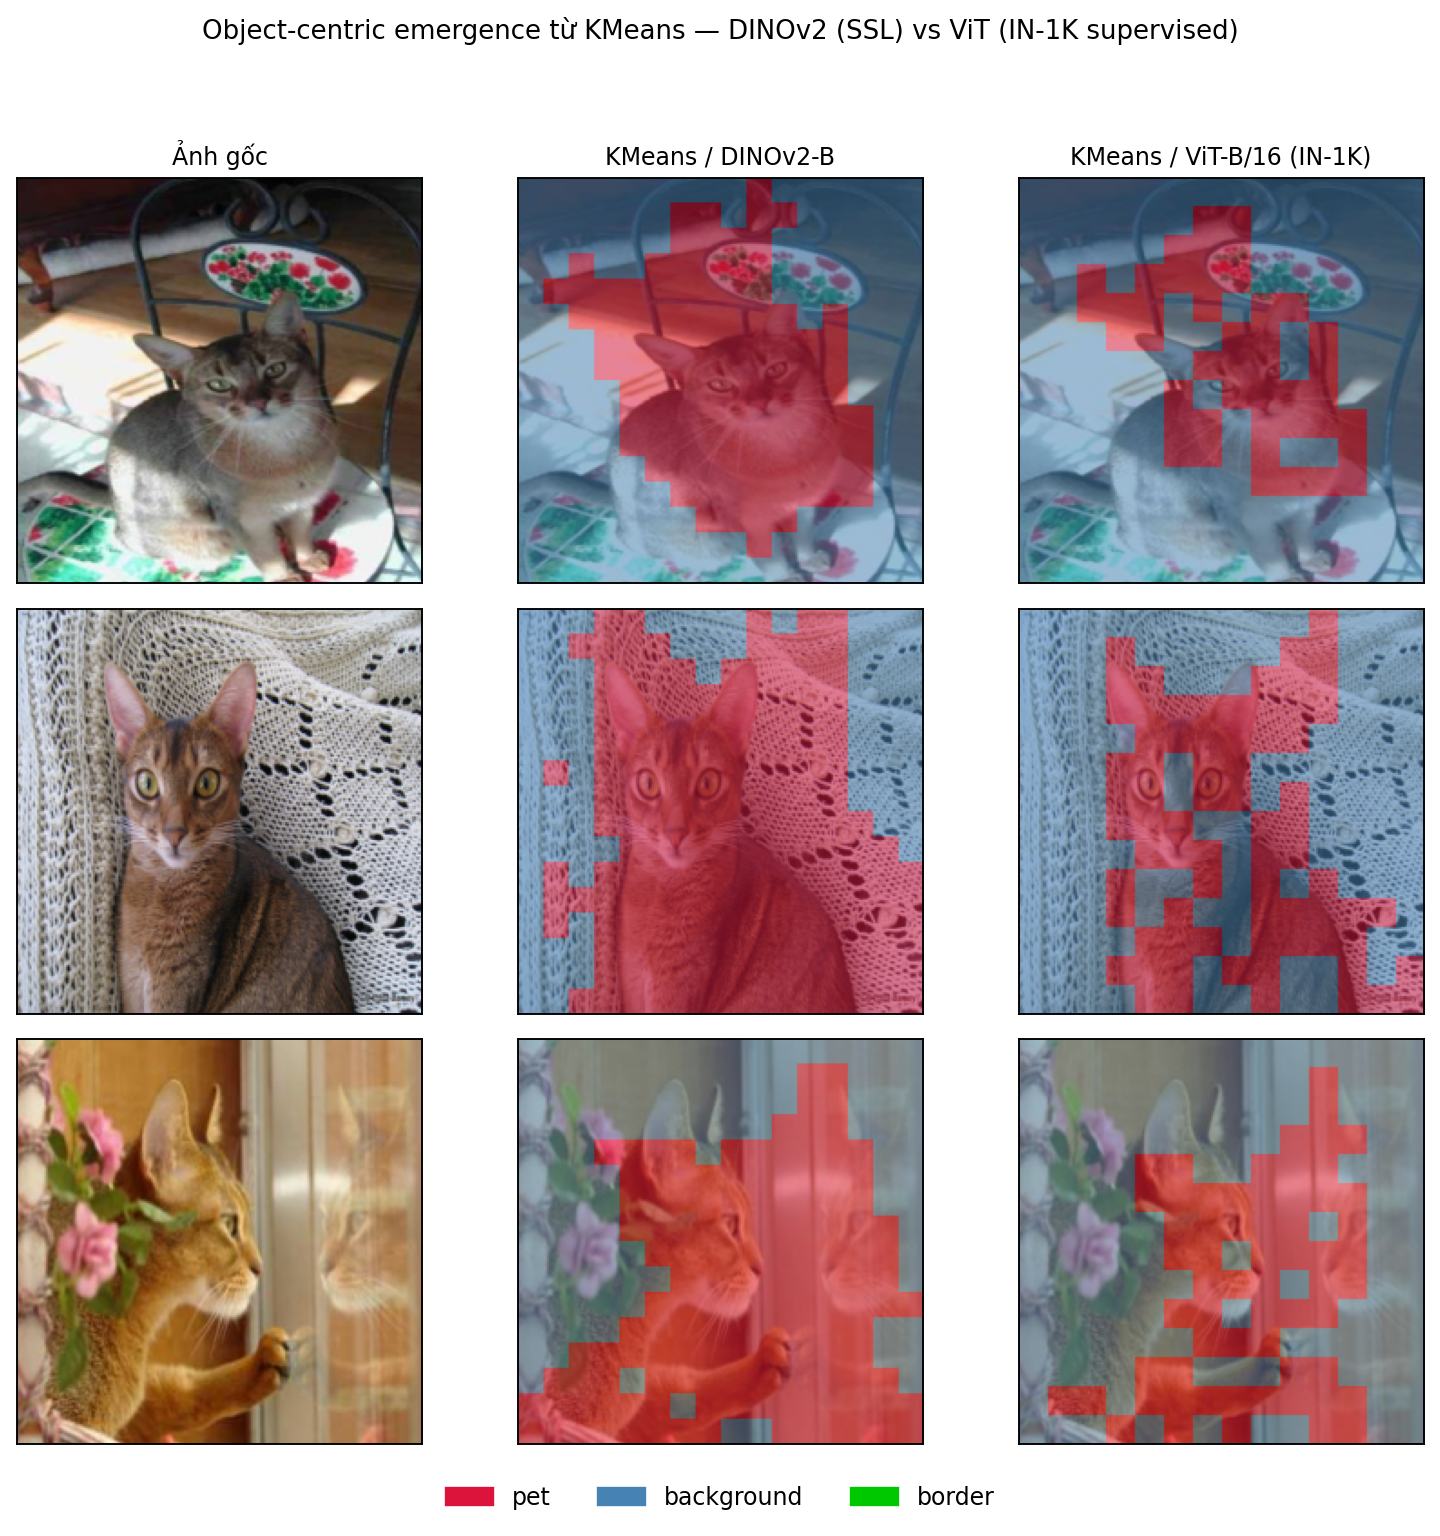
\includegraphics[width=\columnwidth,height=2.8cm,keepaspectratio]{figures/seg_clustering_emergence.png}
            {\tiny \textbf{Hình 13:} KMeans ($k{=}3$): DINOv2 phân biệt foreground/background tự nhiên; ViT-B/16 bị ``vỡ'' thành nhiều mảnh}
            \vspace{0.1cm}
            \begin{exampleblock}{Object-centric emergence}
                \small DINOv2 \textbf{không dùng nhãn nào} vẫn sinh ra ranh giới đối tượng rõ nét --- tính chất tự phát từ SSL quy mô lớn
            \end{exampleblock}
            \begin{alertblock}{Failure case}
                \small Quả bóng nâu bị nhầm vào lớp \textit{pet} do texture tương đồng --- mô hình chỉ thấy những gì có trong reference
            \end{alertblock}
        \end{column}
    \end{columns}
\end{frame}

% ============================================================
\section{Đánh giá \& Ứng dụng}
% ============================================================

% ============================================================
% SLIDE 19: ĐIỂM MẠNH & HẠN CHẾ
% ============================================================
\begin{frame}[t,shrink=15]{Đánh giá Tổng hợp: Điểm mạnh \& Hạn chế}
    \begin{columns}[t]
        \begin{column}{0.48\textwidth}
            \begin{exampleblock}{Điểm mạnh}
                \begin{itemize}
                    \item \textbf{Out-of-the-box features} mạnh: linear probe hội tụ nhanh trên domain mới
                    \item \textbf{Patch features} chất lượng cao: dense task không cần gradient
                    \item \textbf{Object-centric emergence}: clustering tự phát sinh ranh giới đối tượng
                    \item \textbf{DINOv2-S đủ tốt}: 21M params, phù hợp thiết bị hạn chế tài nguyên
                    \item Pipeline \textbf{rất nhẹ}: few-shot (10 ảnh) hoặc zero-shot (clustering)
                \end{itemize}
            \end{exampleblock}
        \end{column}
        \begin{column}{0.48\textwidth}
            \begin{alertblock}{Hạn chế}
                \begin{itemize}
                    \item \textbf{Chi phí pretrain}: hàng nghìn GPU-hours --- không thể tái tạo độc lập
                    \item \textbf{Patch resolution}: class \textit{border} IoU thấp --- không phân giải pixel-level
                    \item \textbf{Thiếu interpretability}: cần Grad-CAM / Attention Maps cho ứng dụng y tế
                    \item \textbf{Phụ thuộc reference}: reference không đa dạng $\to$ tổng quát hóa kém
                    \item \textbf{Bias dữ liệu}: web data có bias địa lý và nhân khẩu học
                \end{itemize}
            \end{alertblock}
        \end{column}
    \end{columns}
\end{frame}

% ============================================================
% SLIDE 20: ỨNG DỤNG THỰC TẾ
% ============================================================
\begin{frame}[t,shrink=15]{Khả năng Ứng dụng Thực tế}
    \begin{columns}[t]
        \begin{column}{0.48\textwidth}
            \begin{block}{Y tế (Medical Imaging)}
                \small
                \begin{itemize}
                    \item Phân loại bệnh lý với rất ít nhãn (few-shot linear probe)
                    \item Phân đoạn tổn thương zero-shot từ vài ảnh mẫu
                    \item Giảm mạnh chi phí gán nhãn pixel-level bởi chuyên gia
                    \item \textit{Đã kiểm chứng: SkinCancerMNIST 80\% accuracy không nhãn pretrain}
                \end{itemize}
            \end{block}
            \vspace{0.2cm}
            \begin{block}{Nông nghiệp thông minh}
                \small
                \begin{itemize}
                    \item Phát hiện sâu bệnh trên lá từ ảnh drone
                    \item Phân đoạn vùng bệnh với rất ít mẫu
                    \item DINOv2-S phù hợp triển khai trên thiết bị di động, edge devices
                \end{itemize}
            \end{block}
        \end{column}
        \begin{column}{0.48\textwidth}
            \begin{block}{Xe tự lái / Robot}
                \small
                \begin{itemize}
                    \item Segmentation ngữ nghĩa không cần fine-tune
                    \item Depth estimation từ frozen patch features
                    \item Hiểu cấu trúc không gian phức tạp
                    \item DINOv2-S phù hợp cho embedded systems
                \end{itemize}
            \end{block}
            \vspace{0.2cm}
            \begin{block}{Tìm kiếm \& Truy xuất ảnh}
                \small
                \begin{itemize}
                    \item CLS features + KoLeo $\to$ semantic search chất lượng cao
                    \item Ứng dụng: e-commerce, digital asset management, kho ảnh y tế
                    \item Không cần gán nhãn, dùng ngay frozen embedding
                \end{itemize}
            \end{block}
        \end{column}
    \end{columns}
\end{frame}

% ============================================================
% SLIDE 21: KẾT LUẬN
% ============================================================
\begin{frame}[t,shrink=15]{Kết luận}
    \begin{block}{Những điều DINOv2 chứng minh được}
        \begin{enumerate}
            \item \textbf{SSL có thể cạnh tranh với weakly-supervised learning} nếu dữ liệu curated tốt và scale đủ lớn --- xóa bỏ quan niệm SSL kém hơn text-guided pretraining
            \vspace{0.1cm}
            \item \textbf{Patch-level features từ SSL} chứa thông tin không gian đủ mạnh cho dense tasks (segmentation, depth) mà không cần fine-tune backbone
            \vspace{0.1cm}
            \item \textbf{Object-centric emergence}: đặc tính tự phát giúp clustering không nhãn vẫn tạo ra ranh giới đối tượng rõ nét
            \vspace{0.1cm}
            \item \textbf{Frozen visual foundation model} không phụ thuộc caption/nhãn --- tiền đề cho AI đa phương thức thế hệ tiếp theo
        \end{enumerate}
    \end{block}
    \vspace{0.15cm}
    \begin{center}
        \begin{tikzpicture}
            \node[draw=uetblue,fill=uetgold!30,rounded corners=6pt,inner sep=8pt,
                  text width=11cm,align=center] {
                \textbf{Công thức thành công của DINOv2:}\\[3pt]
                \large Dữ liệu curated \ $+$ \ SSL recipe ổn định \ $+$ \ Scale hiệu quả
            };
        \end{tikzpicture}
    \end{center}
\end{frame}

% ============================================================
% SLIDE 22: Q&A
% ============================================================
\begin{frame}[plain]
    \begin{tikzpicture}[remember picture, overlay]
        \fill[uetblue!95] (current page.north west) rectangle (current page.south east);
    \end{tikzpicture}
    \begin{center}
        \vspace{3cm}
        {\color{white}\Large\bfseries Cảm ơn thầy/cô và các bạn đã lắng nghe!}
    \end{center}
\end{frame}

\end{document}
